\documentclass[../main.tex]{subfiles}

%\graphicspath{{\subfix{../images/}}}

\begin{document}


\begin{align}
    \left(\int_{-\infty}^\infty dx e^{-x^2}\right)^2
    &=\int_{-\infty}^\infty dx e^{-x^2} \cdot \int_{-\infty}^\infty dy e^{-y^2}\\
    &=\int_{\mathbb{R}^2}e^{-(x^2+y^2)}dx\,dy\\
    &=\int_0^{2\pi}\int_0^{2\pi}e^{-r^2}r dr \\
    &=-2\pi\left.\frac{e^{-r^2}}{2}\right|^\infty_0=\pi
\end{align}

\section{Common integrals}
\begin{align}
    \int_{-\infty}^\infty dx e^{-ax^2}&=\sqrt{\frac{\pi}{a}} \qquad a>0, a\in\mathbb{R}\\
    \int_{-\infty}^\infty dx e^{-ax^2+bx+c}&=\sqrt{\frac{\pi}{a}}e^{\frac{b^2}{4a}+c} \qquad a>0, a,b,c\in\mathbb{R}\\
    \int_{-\infty}^\infty dx e^{iax^2}&=\sqrt{\frac{\pi}{a}}e^{\frac{i\pi}{4}} \qquad a>0, a\in\mathbb{R}\\
%    
\text{modified Bessel}\quad K_0(a\beta)&=\int_0^\infty dx \frac{\cos(ax)}{\sqrt{\beta^2+x^2}} \qquad \text{Gradshteyn, Ryzhik 7ed (3.754)}\\
\text{modified Bessel}\quad K_1(a\beta)&=\frac{1}{\beta}\int_0^\infty dx \frac{x\sin(ax)}{\sqrt{\beta^2+x^2}}
\end{align}



\section{Common Fourier integrals}
\begin{align}
    \int_{-\infty}^\infty dy e^{-ay^2}e^{-iby}&=\sqrt{\frac{\pi}{a}}e^{-\frac{b^2}{4a}} \qquad a>0, a,b\in\mathbb{R}\\
    \int_{-\infty}^\infty dy e^{iay^2}e^{-iby}&=\sqrt{\frac{\pi}{a}}e^{\frac{i}{4}\left(\pi-\frac{b^2}{a}\right)} \qquad a>0, a,b\in\mathbb{R}\\
    \int_{-\infty}^\infty dy e^{-(a+ic)y^2}e^{-iby}&=\sqrt{\frac{\pi}{a+ic}}e^{-\frac{b^2}{4(a+ic)}} \qquad a>0, a,b,c\in\mathbb{R}\\
    &=\sqrt{\frac{\pi}{a^2+c^2}}\sqrt{a-ic}\,e^{-\frac{b^2}{4(a^2+c^2)}(a-ic)}
\end{align}

\section{Residue theorem}
\begin{align}
\int_\Gamma f=2\pi i\sum_{a\in D_\text{Singu}}\text{ind}_\Gamma(a)\,\text{Res}_af
\end{align}
Winding number $\text{ind}_\Gamma(a)$, Residue $\text{Res}_af=c_{-1}$ from Laurent series at singularity $a$
\begin{align}
f(z)=\sum_{n=-\infty}^\infty c_n(z-a)^n
\end{align}


\section{Common contour integrals}
\begin{align}
G(t-t')&=-\frac{1}{2\pi}\int_{-\infty}^{+\infty}dE\frac{e^{-iE(t-t')}}{E^2-\omega^2+i\epsilon}=\frac{i}{2\omega}e^{i\omega|t|}\qquad\text{Sredniki (7.12)}\\
D(x-y)&=\frac{4\pi}{(2\pi)^3}\int_{0}^{\infty} dp\frac{p^2 e^{i\sqrt{p^2+m^2}t}}{2\sqrt{p^2+m^2}}=\frac{1}{4\pi^2}\int_m^\infty dE\sqrt{E^2-m^2}e^{iEt}\qquad \text{PS (2.51)}\\
D(x-y)&=\frac{-i}{2(2\pi)^2r}\int_{-\infty}^{+\infty} dp\frac{p e^{ipr}}{\sqrt{p^2+m^2}}=\frac{1}{4\pi^2 r}\int_m^\infty d\rho\frac{\rho e^{-\rho r}}{\sqrt{\rho^2-m^2}}\qquad\text{PS (2.52)}\\
V(r)&=\frac{1}{(2\pi)^2ir}\int_{-\infty}^\infty dp\frac{p e^{ipr}}{p^2+m^2}=\frac{1}{4\pi r}e^{-mr}\qquad\text{PS (4.126)}
\end{align}

\section{Feynman integral tricks}
\subsection{First example}
\begin{align}
\int_{0}^{\infty}\frac{e^{-t^2(x^2+1)}}{x^2+1}dx
\end{align}



\subsection{Second example}
We are trying to evaluate the integral without using contour integrals
\begin{align}
\int_{-\infty}^{\infty}\frac{\log(x^4+1)}{x^2+1}
&=2\int_0^{\infty}\frac{\log(x^4+1)}{x^2+1}dx\\
&=2\int_0^{\infty}\frac{\log[(x^2-i)(x^2+i)]}{x^2+1}dx\\
&=2\int_0^{\infty}\frac{\log(x^2-i)}{x^2+1}+\frac{\log(x^2+i)}{x^2+1}dx\\
&=2\left(I(-i)+I(i)\right)
\end{align}
Now the trick - come up with a parameter $t$ inside the integral
\begin{align}
I(t)&=\int_0^{\infty}\frac{\log(x^2+t)}{x^2+1}dx\\
I(0)&=\int_0^{\infty}\frac{2\log(x)}{x^2+1}dx\\
&\overset{x=1/u}{=}\int_\infty^0\frac{2\log(1/u)}{1/u^2+1}\frac{-1}{u^2}du\\
&=(-1)^2\int_0^{\infty}\frac{-2\log(u)}{1+u^2}du\\
&=-I(0)=0
\end{align}
and differentiate with respect to $t$ (\textcolor{blue}{without checking if are allowed to switch the integral and the differentiation})
\begin{align}
\frac{dI}{dt}
&=\int_0^{\infty}\frac{1}{x^2+1}\frac{1}{x^2+t}dx\\
&=\int_0^{\infty}\frac{1/(t-1)}{x^2+1}+\frac{1/(1-t)}{x^2+t}dx\\
&=\left.\frac{\arctan x}{t-1}\right|_0^\infty-\left.\frac{\arctan \frac{x}{\sqrt{t}}}{(t-1)\sqrt{t}}\right|_0^\infty\\
&=\frac{\pi}{2}\frac{1}{t-1}\frac{\sqrt{t}-1}{\sqrt{t}}\\
&=\frac{\pi}{2}\frac{1}{\sqrt{t}(1+\sqrt{t})}
\end{align}
and now we can integrate
\begin{align}
I(t)
&=\frac{\pi}{2}\int\frac{1}{\sqrt{t}(1+\sqrt{t})}dt\\
&\overset{u=\sqrt{t}}{=}\frac{\pi}{2}\int\frac{1}{u(1+u)}2u\,du\qquad\frac{du}{dt}=\frac{1}{2\sqrt{t}},\rightarrow dt=2u\,du\\
&=\pi\log(1+u)+c\qquad\text{with}\,I(0)=0\rightarrow c=0\\
&=\pi\log(1+\sqrt{t})
\end{align}
then with $i=e^{i\pi/2+2\pi k}$ and $-i=e^{-i\pi/2+2\pi n}$
\begin{align}
\int_{-\infty}^{\infty}\frac{\log(x^4+1)}{x^2+1}
&=2\left(I(-i)+I(i)\right)\\
&=2\pi\left(\log(1+\sqrt{-i})+\log(1+\sqrt{i})\right)\\
&=2\pi\log[(1+\sqrt{-i})(1+\sqrt{i})]\\
&=2\pi\log[1+\sqrt{-i}+\sqrt{i}+\sqrt{-i^2}]\\
&=2\pi\log[2+\sqrt{-i}+\sqrt{i}]\\
&=2\pi\log[2+e^{-i\pi/4}e^{i\pi n}+e^{i\pi/4}e^{i\pi k}]\\
&=2\pi\log[2+\sqrt{2}]\qquad\text{just setting $n,k=0$ to ensure a real solution}\\
&=\pi\log[(2+\sqrt{2})^2]\\
&=\log[(6+4\sqrt{2})^\pi]\\
\end{align}


\section{Fourier transformation}
Starting from the Fourier integral theorem we have some freedom to distribute the $2\pi$ between back and forth transformation ($a,b\in\mathbb{R}$)
\begin{align}
    F(k)=\sqrt{\frac{|b|}{(2\pi)^{1-a}}}\int_{-\infty}^\infty f(x)e^{ibkx}dx\quad\leftrightarrow\quad f(x)=\sqrt{\frac{|b|}{(2\pi)^{1+a}}}\int_{-\infty}^\infty F(t)e^{-ibkx}dk
\end{align}

\section{Laplace transformation}
Origin: Power series
\begin{align}
\sum_{n=0}^\infty a_n x^n&\simeq A(x)\\
\sum_{n=0}^\infty a(n) x^n&= A(x)
\end{align}
with $n\in\mathbb{N}$ and $a(n)\in\mathbb{R}$. Examples
\begin{align}
a(n)=1\qquad&\rightarrow\qquad A(x)=\frac{1}{1-x}\qquad|x|<1\\
a(n)=\frac{1}{n}\qquad&\rightarrow\qquad A(x)=-\log(1-x)\\
a(n)=\frac{1}{n!}\qquad&\rightarrow\qquad A(x)=e^x
\end{align}
Now extend $n\in\mathbb{N}\rightarrow t\in\mathbb{R}$
\begin{align}
\int_0^\infty a(t) x^t dt&=A(x)\\
\int_0^\infty a(t) e^{\log x\;t} dt&=A(x)\\
\int_0^\infty a(t) e^{-s\;t} dt&=A(e^{s})\\
\int_0^\infty f(t) e^{-st} dt&=F(s)
\end{align}
meaning the Laplace trafo is the continuous analog of the discrete power series.

Now
\begin{align}
Y(s)&=\int_0^\infty f(t)e^{-st}dt
\end{align}
then
\begin{align}
\int_0^\infty f'(t)e^{-st}dt
&=\left.f(t)e^{-st}\right|_0^\infty-\int_0^\infty f(t)(-s)e^{-st}dt\\
&=-f(0)+s\int_0^\infty f(t)e^{-st}dt\\
&=sY(s)-f(0)
\end{align}
\begin{align}
\int_0^\infty f''(t)e^{-st}dt
&=...\\
&=s^2Y(s)-sf'(0)-f(0)
\end{align}

\section{Delta distribution}
\begin{align}
x\delta(x)=0
\delta(ax)=\frac{1}{|a|}\delta(x)
\end{align}

\begin{align}
    \int\delta(x)e^{-ikx}dx&=1\\
    \int e^{ik(x-y)}dk&=2\pi\delta(x-y)
\end{align}
\begin{align}
    \int g(x)\delta(f(x))dx &= \sum_{x_i:f(x_i)=0}\int_{x_i-\epsilon}^{x_i+\epsilon} g(x)\delta(f(x))dx\\
    &= \sum_{x_i}\int_{x_i-\epsilon}^{x_i+\epsilon} g(x)\delta\left(f(x_i)+f'(x_i)(x-x_i)+\frac{1}{2}f''(x_i)(x-x_i)^2+...\right)dx\\
    &= \sum_{x_i}\int_{x_i-\epsilon}^{x_i+\epsilon} g(x)\delta\left(f'(x_i)(x-x_i)\right)dx\\
    &= \sum_{x_i}\int_{(x_i-\epsilon)f'}^{(x_i+\epsilon)f'} g\left(\frac{u}{f'(x_i)}\right)\delta\left(u-f'(x_i)x_i)\right)\frac{1}{f'(x_i)}du\\
    &= \sum_{x_i}\int_{(x_i-\epsilon)|f'|}^{(x_i+\epsilon)|f'|} g\left(\frac{u}{f'(x_i)}\right)\frac{1}{|f'(x_i)|}\delta\left(u-f'(x_i)x_i)\right)du\\
    &= \sum_{x_i} g(x_i)\frac{1}{|f'(x_i)|}
\end{align}
Important restriction: $x_i$ are the {\bf simple} zeros

\section{Bessel functions}
\begin{itemize}
\item Bessel ODE $x^2y''+xy'+(x^2-\nu^2)y=0\qquad \text{Re}\,\nu\ge0$
\begin{align}
y&=c_1y_1+c_2y_2\\
&=\left\{\begin{array}{ll}
c_1J_\nu+c_2J_{-\nu} &  \quad\nu\notin\mathbb{Z}\\
c_1J_\nu+c_2Y_{\nu}  &  \quad\nu=0,1,2,...
\end{array}\right.
\end{align}
\begin{align}
J_\nu(x)&=\left(\frac{x}{2}\right)^\nu\sum_{k=0}^\infty\frac{(-1)^k}{k!\,\Gamma(k+\nu+1)}\left(\frac{x}{2}\right)^{2k}\qquad\text{Bessel function}\\
Y_\nu(x)&=\frac{J_\nu(x)\cos\nu\pi-J_{-\nu}(x)}{\sin\nu\pi}\qquad\text{Neumann/Weber function}\\
Y_n(x)&=\lim_{\alpha\rightarrow n}Y_{\alpha}(x)\\
H_\nu^{(1)}(x)&=J_\nu(x)+iY_\nu(x)\qquad\text{Hankel function 1. kind}\\
H_\nu^{(2)}(x)&=J_\nu(x)-iY_\nu(x)\qquad\text{Hankel function 2. kind}
\end{align}
If $\nu=n$ then 
\begin{align}
J_n
&=\frac{1}{\pi}\int_0^\pi\cos(x\sin\varphi-n\varphi)d\varphi\\
&=\frac{1}{2\pi}\int_{-\pi/2}^{\pi/2}e^{i(x\sin\varphi-n\varphi)}d\varphi
\end{align}

\item Modified Bessel ODE $x^2y''+xy'-(x^2+\nu^2)y=0$
\begin{align}
I_\nu(x)&=i^{-\nu}J_\nu(ix)\\
K_\nu(x)&=\frac{\pi}{2}\frac{I_{-\nu}(x)-I_{\nu}(x)}{\sin\nu\pi}\\
K_n(x)&=\lim_{\alpha\rightarrow n}K_{\alpha}(x)\\
\end{align}
If $\text{Re}\,x>0$ then 
\begin{align}
K_n=\int_0^\pi e^{-x\cosh t}\cosh\nu t\,dt
\end{align}

\end{itemize}


\section{\texorpdfstring{$\Gamma,\zeta $}{TEXT} function}
\begin{align}
    \Gamma(s)&=\int_0^\infty t^{s-1}e^{-t} dt\\
    \zeta(s)&=\sum_{n=1}^\infty\frac{1}{n^s}
\end{align}
then with $t/n=x$ and $dx=dt/n$
\begin{align}
	\zeta(s)\Gamma(s)
	&=\sum_{n=1}^\infty\int_0^\infty \frac{1}{n^s}t^{s-1}e^{-t} dt\\
	&=\sum_{n=1}^\infty\int_0^\infty \frac{1}{n^s}t^{s-1}e^{-t} n\,dx\\
	&=\sum_{n=1}^\infty\int_0^\infty \frac{t^{s-1}}{n^{s-1}}e^{-nx} dx\\
	&=\int_0^\infty x^{s-1}\sum_{n=1}^\infty e^{-nx} dx\\
	&=\int_0^\infty \frac{x^{s-1}}{e^{x}-1} dx\\
\zeta(s)&=\frac{1}{\Gamma(s)}\int_0^\infty \frac{x^{s-1}}{e^{x}-1} dx
\end{align}



\section{\texorpdfstring{$n$}{TEXT}-dimensional unit spheres}
\begin{align}
    \pi^{n/2}
    &=\left(\int_{-\infty}^\infty dt e^{-t^2}\right)^n\\
    &=\int_{R^n} e^{-|x|^2}dx\\
    &=\int_0^\infty\int_{\omega_n}e^{-r^2}r^{n-1}dr\,ds\\
    &=\int_{\omega_n}ds\cdot\int_0^\infty e^{-r^2}r^{n-1}dr\\
    &=|\omega_n|\cdot\frac{1}{2}\int_0^\infty e^{-\rho}\rho^{\frac{n}{2}-1}d\rho\\
    &=|\omega_n|\cdot\frac{1}{2}\Gamma\left(\frac{n}{2}\right)
\end{align}
Therefore
\begin{align}
|\omega_n| &= \frac{2\pi^{n/2}}{\Gamma\left(\frac{n}{2}\right)}\\
V_n 
&=|\omega_n|\int_0^1r^{n-1}dr\\
&=\frac{|\omega_n|}{n}
\end{align}

\section{Vector Analysis}
Identities
\begin{align}
\nabla\times\nabla\phi&\equiv0\\
\nabla\cdot\nabla\times\mathbf{A}&\equiv\mathbf{0}\\
\nabla\times\nabla\times\mathbf{A}&=\nabla(\nabla\cdot\mathbf{A})-\triangle\mathbf{A}
\end{align}
Gauss and Stokes Theorem
\begin{align}
\oint_{\partial V}\mathbf{A}\cdot
d\mathbf{S}&=\int_V\nabla\cdot\mathbf{A}\,dV\\
\oint_{\partial S}\mathbf{A}\cdot
d\mathbf{r}&=\int_S(\nabla\times\mathbf{A})\cdot d\mathbf{S}
\end{align}
Helmholtz-Hodge decomposition
\begin{align}
\mathbf{E}&=\mathbf{E}_\parallel+\mathbf{E}_\perp\\
\nabla\times\mathbf{E}_\parallel&=0\\
\nabla\cdot\mathbf{E}_\perp&=0
\end{align}
With
\begin{align}
-\frac{1}{4\pi}\triangle\frac{1}{|\mathbf{x}-\mathbf{x}'|}&=\delta(\mathbf{x}-\mathbf{x}')\\
\triangle\mathbf{E}&=\nabla(\nabla\cdot\mathbf{E})-\nabla\times\nabla\times\mathbf{E}
\end{align}
we can construct
\begin{align}
\mathbf{E}(\mathbf{x})
&=\int \mathbf{E}(\mathbf{x}') \delta(\mathbf{x}-\mathbf{x}')dx'\\
&=-\frac{1}{4\pi}\int \mathbf{E}(\mathbf{x}')\triangle\frac{1}{|\mathbf{x}-\mathbf{x}'|}dx'\\
&=-\frac{1}{4\pi}\triangle\int \mathbf{E}(\mathbf{x}')\frac{1}{|\mathbf{x}-\mathbf{x}'|}dx'\\
&=-\frac{1}{4\pi}\nabla\int \mathbf{E}(\mathbf{x}')\nabla\cdot\frac{1}{|\mathbf{x}-\mathbf{x}'|}dx'+\frac{1}{4\pi}\nabla\times\int \mathbf{E}(\mathbf{x}')\nabla\times\frac{1}{|\mathbf{x}-\mathbf{x}'|}dx'\\
\end{align}

\section{Laplace operator}
\begin{align}
    \nabla\cdot X&=\frac{1}{\sqrt{|g|}}\partial_i\left(\sqrt{|g|}X^i\right)\\
    (\nabla f)^i&=g^{ij}\partial_jf\\
    \triangle f &= \nabla\cdot\nabla f\\
    &=\frac{1}{\sqrt{|g|}}\partial_i\left(\sqrt{|g|} g^{ij}\partial_jf \right)\\
    &= \sum_i \frac{\partial^2}{\partial x_j^2}
\end{align}

\begin{align}
    \frac{\partial}{\partial x_i}\frac{\partial f}{\partial x_i}
    &=\frac{\partial}{\partial x_i}\left(\frac{\partial y_j}{\partial x_i}\frac{\partial f}{\partial y_j}\right)\\
    &=\frac{\partial y_k}{\partial x_i}\frac{\partial}{\partial y_k}\left(\frac{\partial y_j}{\partial x_i}\frac{\partial f}{\partial y_j}\right)\\
    &=\frac{\partial^2 y_j}{\partial x_i^2}\frac{\partial f}{\partial y_j} + \frac{\partial y_j}{\partial x_i}\frac{\partial y_k}{\partial x_i}\frac{\partial^2 f}{\partial y_j\partial y_k}\\
\end{align}
With $f=f(r)$ and $r=\sqrt{x_1^2+...+x_n^2}$ we have
\begin{align}
    \triangle f(r)
    &=\sum_i \frac{r-x_i \frac{x_i}{r}}{r^2}\frac{\partial f}{\partial r}+\frac{x_i^2}{r^2}\frac{\partial^2 f}{\partial r^2}\\
    &= \frac{nr-r}{r^2}\frac{\partial f}{\partial r}+\frac{r^2}{r^2}\frac{\partial^2 f}{\partial r^2}\\
    &= \frac{(n-1)}{r}\frac{\partial f}{\partial r}+\frac{\partial^2 f}{\partial r^2}
\end{align}

\section{ODE solving strategies}
\subsection{Special ODEs}
\begin{tabular}{lrl}
Bernoulli       & $y'+p(x)y+q(x)y^n=0$			&\\
Ricatti         & $y'+p(x)y+q(x)y^2=r(x)$		&\\
d'Alembert      & $y=x\cdot g(y')+h(y')$		&\\
Exact           & $M(x,y)+N(x,y)y'=0 \quad (\partial_yM=\partial_xN)$	&\\
                & \\
Airy            & $y''-xy=0$					&\\
Bessel          & $x^2y''+xy'+(x^2-\nu^2)y=0$	& $\text{Re}
\,\nu\ge0$\\
modified Bessel & $x^2y''+xy'-(x^2+\nu^2)y=0$	&\\
Hermite         & $y''-2xy'+2ny=0$				& $n=0,1,2,3,...$\\
Laguerre        & $xy''+(1-x)y'+ny=0$			& $n=0,1,2,3,...$\\
Legendre		& $(1-x^2)y''-2xy'+n(n+1)y=0$	& $n=0,1,2,3,...$\\
Weber Hermite   & $y''+\left(\nu+\frac{1}{2}-\frac{1}{4}x^2\right)y=0$
\end{tabular}

\newpage
\subsection{1st order ODE}
\begin{enumerate}
\item Is separable $y'=g(x)h(y)\quad\rightarrow\quad \int\frac{dy}{h(y)}=\int g(x)dx$ - done.
\item Is linear homogen $y'+f(x)y=0$ go to 1.
\begin{align}
y(x)=Ce^{-\int f(x)dx}
\end{align}
\item Is linear inhomogen $y'+f(x)y=g(x)$ general solution
\begin{align}
y(x)&=y_\text{hom}(x)+y_\text{spec}(x)\\
y_\text{hom}(x)&=Ce^{-\int f(x)dx}\\
y_\text{spec}(x)&=C(x)e^{-\int f(x)dx}\\
&\rightarrow C(x)'e^{-\int f(x)dx}-f(x)C(x)e^{-\int f(x)dx}+f(x)C(x)e^{-\int f(x)dx}=g(x)\\
&\rightarrow C(x)'=g(x)e^{\int f(x)dx}\\
&\rightarrow C(x)=\int g(x)e^{\int f(x)dx}dx+c_1\\
y(x)&=Ce^{-\int f(x)dx}+\left(\int g(x)e^{\int f(x)dx}dx+c_1\right)e^{-\int f(x)dx}
\end{align}
solve homogen (go to 2) then variation of constants.
\item Is linear Bernoulli $y'+f(x)y+g(x)y^n=0$ divide by $y^n$ and subs $z=\frac{1}{y^{n-1}}$ then go to 3.
\item Is linear Ricatti $y'+f(x)y+g(x)y^2=r(x)$ substitude with $y=Q\frac{w'}{w}$ to linearize it
\begin{align}
Q'\frac{w'}{w}+\frac{Qw''}{w}-\frac{Q{w'}^2}{w^2}+fQ\frac{w'}{w}+gQ^2\frac{{w'}^2}{w^2}&=r\\
Q'\frac{w'}{w}+\frac{Qw''}{w}+\left(gQ-1\right)Q\frac{{w'}^2}{w^2}+fQ\frac{w'}{w}&=r\qquad gQ-1=0\\
Q'w'+Qw''+fQw'&=rw\\
w''+\frac{Q'+fQ}{Q}w'-\frac{r}{Q}w&=0\quad Q=1/g, Q'=-1/g^2\\
w''+\left(-\frac{1}{g}+f\right)w'-rgw&=0
\end{align}
\item Is exact $M(x,y)+N(x,y)y'=0$ with $M_y=N_y$ then solution $\Phi(x,y)=C$ because
\begin{align}
0=\frac{d\Phi(x,y)}{dx}&=\frac{\partial\Phi}{\partial x}+\frac{\partial\Phi}{\partial y}\frac{dy}{dx}\\
d\Phi&=M(x,y)dx+N(x,y)dy\\
\Phi(x,y)&=\int_{y_0}^yN(x,v)dv+\int_{x_0}^xM(u,y)du
\end{align}
or easier
\begin{align}
\frac{\partial\Phi}{\partial x}=M\quad\rightarrow\quad\Phi=\int M dx+G(y)\quad\rightarrow\quad\frac{\partial\Phi}{\partial y}=N
\end{align}
\item If nothing works try if of form $y'=f\left(\frac{y}{x}\right)$ and subs $z=y/x$ and go to 1.

\item If still nothing works try $y=u(x)\cdot v(x)$
\end{enumerate}

\subsection{2nd order ODE}
Linear homegeneous equation - we can simplify
\begin{align}
&y''+a(x)y'+b(x)y=0 \quad\rightarrow\quad y=f(x)u\\
&f''u+2f'u'+u''+a(f'u+fu')+bfu=0\\
&u''+(2f'+af)u'+(f''+af'+bf)u=0\quad\rightarrow\quad 2f'+af=0\\
&u''+q(x)u=0
\end{align}
Why is it hard to solve 2nd order ODE
\begin{align}
y''+a(x)y'+b(x)y=0\\
(D^2+aD+b)y=0
\end{align}
Lets try to factorize the differential operator
\begin{align}
(D+A)(D+B)y=0\\
(D^2+(A+B)D+B'+AB)y=0
\end{align}
Once we know $A$ and $B$ we can solve
\begin{align}
(D+B)y\equiv w\\
w'+Aw=0 \quad\text{(very simple to solve for $w$)}\\
y'+by=w \quad\text{(simple to solve for $y$)}
\end{align}
But how to find $A$ and $B$
\begin{align}
A+B=a, \quad B'=-AB+b\\
\rightarrow B'=-aB+B^2+b
\end{align}
which gives the Riccati equation - but linearizing it leads back to the same linear, homogeneous 2nd order equation (which we started with).

\begin{enumerate}
\item Is inhomogeneous equation with constant coefficients $ay''+by'+cy=r(x)$
\begin{align}
a[s^2Y-sy(0)-y'(0)]+b[sY-y(0)]+cY&=\mathcal{L}(r(x))\\
(as^2+bs+c)Y-asy(0)-ay'(0)-by(0)&=\mathcal{L}(r(x))\\
Y=\frac{\mathcal{L}(r(x))+(as+b)y(0)+ay'(0)}{as^2+bs+c}
\end{align}

\end{enumerate}
... write me ...

\subsection{n-th order ODE}
\begin{enumerate}
\item Linear homogen $c_ny^{n}+...+c_{2}y''+c_{1}y'+c_{0}y=0$ ansatz $y=e^{\alpha x}$ then solve polynom for $\alpha$,  for repeated root $\alpha_1$ try $y=xe^{\alpha_1 x}, x^2e^{\alpha_1 x}, ...$
\end{enumerate}




\section{Greenfunctions and ODEs}
\subsection{Harmonic Oscillator}
\begin{align}
\ddot{G}(t-t')+2\gamma\dot{G}(t-t')+\omega_0^2G(t-t')=\delta(t-t')
\end{align}
with $G(t-t')=(2\pi)^{-1/2}\int e^{i\omega (t-t')}y(\omega)d\omega$
\begin{align}
\frac{1}{\sqrt{2\pi}}\int e^{i\omega (t-t')}\left((i\omega)^2y+2\gamma(i\omega)y+\omega_0y\right)d\omega=\frac{1}{2\pi}\int e^{i\omega(t-t')}d\omega
\end{align}
then
\begin{align}
y(\omega)&=\frac{1}{\sqrt{2\pi}}\frac{1}{\omega_0^2-\omega^2+2i\gamma\omega}\\
G(t-t')&=\frac{1}{2\pi}\int \frac{e^{-i\omega(t-t')}}{\omega_0^2-\omega^2+2i\gamma\omega}d\omega
\end{align}
and the general solution is given by
\begin{align}
\ddot{x}(t)+2\gamma\dot{x}(t)+\omega_0^2x(t)=f(t)\quad\rightarrow\quad
x(t)=\int G(t-t')f(t)
\end{align}

\section{PDEs}
\subsection{Transport equation $u_t+cu_x=0$}
Imagine $x=x(t)$ so $u(x,t)=u(x(t),t)$, then formally we write
\begin{align}
\frac{du}{dt}&=\frac{\partial u}{\partial t}+\frac{\partial u}{\partial x}\frac{\partial x}{\partial t}\\
&=u_t+u_x\frac{\partial x}{\partial t}\\
u_t+cu_x=0\qquad &\Leftrightarrow \qquad \frac{du}{dt}=0,\quad \frac{\partial x}{\partial t}=c
\end{align}
Solving the two ODEs
\begin{align}
\frac{\partial x}{\partial t}=c\quad&\rightarrow\quad x=ct+x_0\\
\frac{du}{dt}=0\quad&\rightarrow\quad u(x=ct+x_0,t)=u(x=x_0,t)\\
&\rightarrow\quad u(x,t)=u(x-ct,0)=u_0(x-ct)
\end{align}

\subsection{Transport equation $u_t+cu_x=g(t)$}
\begin{align}
u(x,t)=u_0(x,t)+\frac{1}{c}\int_{x-ct}^x g\left(t+\frac{\xi-x}{c}\right)d\xi
\end{align}

\subsection{Transport equation $u_t+cu_x=g(x,t)$}
\begin{align}
u(x,t)=u_0(x,t)+\frac{1}{c}\int_{x-ct}^x g\left(\xi,t+\frac{\xi-x}{c}\right)d\xi
\end{align}

\section{Greenfunctions and PDEs}
The Greensfunction $G(x,y)$ for a general PDE $D_x u(x) = f(x)$ is defined by
\begin{align}
    D_x G(x,y) = \delta(x-y).
\end{align}
This means that general solution of the PDE can be expressed as
\begin{align}
    u(x)=\int G(x,y)f(y)dy
\end{align}
because
\begin{align}
    D_x u(x)
    &=D_x \int G(x,y)f(y)dy\\
    &=\int D_x G(x,y)f(y)dy\\
    &=\int \delta(x-y) f(y)dy\\
    &=f(x)
\end{align}

\newpage
\subsection{Poisson equation \texorpdfstring{$\triangle u(x) = f(x)$}{TEXT}}
        
The $n$-dimensional Fourier transform of $\triangle_x G(x,y) = \delta(x-y)$ and integration by parts gives
    \begin{align}
        \frac{1}{(2\pi)^{n/2}}\int d^nx\,\triangle_x G(x,y) e^{-ikx}&=\frac{1}{(2\pi)^{n/2}}\underbrace{\int d^nx\,\delta(x-y) e^{-ikx}}_{=e^{-iky}}\\
        \frac{1}{(2\pi)^{n/2}}\int d^nx\, G(x,y) (-ik)^2 e^{-ikx}&=\frac{1}{(2\pi)^{n/2}}e^{-iky}\\
        (-ik)^2g(k)&=\frac{1}{(2\pi)^{n/2}}e^{-iky}\\
        &\rightarrow g(k)=-\frac{1}{(2\pi)^{n/2}}\frac{1}{k^2}e^{-iky}
    \end{align}
    we can now use the Fourier transform of the Greensfunction and transform back.
    \begin{itemize}
        \item Case $n=1$: The function has a pole at $k=0$ and the Laurent series is given by
        \begin{align}
            \frac{e^{ik(x-y)}}{k^2}=\frac{1}{k^2}+i(x-y)\frac{1}{k}-\frac{(x-y)^2}{2}-\frac{i(x-y)^3}{6} k + ...
        \end{align}
        with $\text{Res}=i(x-y)$. We can now use the residue theorem to evaluate the integral
        \begin{align}
            G(x,y)&=-\frac{1}{\sqrt{2\pi}}\frac{1}{\sqrt{2\pi}}\int_{-\infty}^\infty dk\; \frac{e^{ik(x-y)}}{k^2}=-\frac{1}{2\pi}\int_{C_1} dk\; \frac{e^{ik(x-y)}}{k^2}\\
            &=-\frac{1}{2\pi}\left(\underbrace{\int_C dk\; \frac{e^{ik(x-y)}}{k^2}}_{=2\pi i\;\text{Res}} - \underbrace{\int_{C_2} dk\; \frac{e^{ik(x-y)}}{k^2}}_{=0}\right)\\
            &=(x-y)
        \end{align}
    
        \begin{center}
        \begin{tikzpicture}[decoration={markings,
            mark=at position 0.5cm with {\arrow[line width=1pt]{>}},
            mark=at position 2cm with {\arrow[line width=1pt]{>}},
            mark=at position 7.85cm with {\arrow[line width=1pt]{>}},
            mark=at position 9cm with {\arrow[line width=1pt]{>}}
            }
            ]
            % The axes
            \draw[help lines,->] (-4,0) -- (4,0) coordinate (xaxis);
            \draw[help lines,->] (0,-1) -- (0,4) coordinate (yaxis);
            
            
            \node at (0,0) {$\times$};
            
            % The path
            %\path[draw,line width=0.8pt,postaction=decorate] (1,0) node[below] {$\epsilon$} -- (2,0) node[below] {$r$} arc (0:180:2) -- (-1,0) arc (180:0:1);
            
            \path[draw,line width=0.8pt,postaction=decorate] (0.5,0)  -- (3,0) node[below] {$R$} arc (0:180:3) node[below] {$-R$} -- (-0.5,0) node[above]{$-\epsilon$} arc (180:360:.5);
            
            % The labels
            \node[below] at (xaxis) {$\Re(k)$};
            \node[left] at (yaxis) {$\Im(k)$};
            \node[above right] {$O$};
            \node at (1.5,.4) {$C_{1}$};
            \node at (2,3) {$C_{2}$};
        \end{tikzpicture}
        \end{center}
        \item Case $n=2$:
        \begin{align}
            G(x,y)&=-\frac{1}{2\pi}\frac{1}{2\pi}\int_{-\infty}^\infty \int_{-\infty}^\infty dk_1 dk_2\; \frac{e^{i(k_1(x_1-y1)+k_2(x_2-y2))}}{k_1^2+k_2^2}\\
            &=-\frac{1}{4\pi^2}\int_{0}^\infty \int_{0}^{2\pi} dk\;d\phi\; \frac{e^{ik |x-y|\cos\phi}}{k^2}k\\
            &=\frac{1}{2\pi}\int_{0}^\infty dk \frac{1}{k}\frac{1}{2\pi}\int_{0}^{2\pi} d\phi\; e^{ik |x-y|\cos\phi}\\
            &=\frac{1}{2\pi}\int_{0}^\infty dk \; \frac{J_0(k|x-y|)}{k}=-\frac{1}{2\pi}\int_{0}^{\infty|x-y|} dk' \; \frac{J_0(k')}{k'}
        \end{align}
        \textcolor{red}{The last integral diverges but we try a nasty trick (?!?)}
        \begin{align}
            \frac{dG}{dx}&=-\frac{1}{2\pi}\frac{d}{dx}\int_{0}^{\infty} dk \; \frac{J_0(k|x-y|)}{k}\\
            &=-\frac{1}{2\pi}\int_{0}^{\infty} dk \; J_1(k|x-y|)\\
            &=-\frac{1}{2\pi}\frac{1}{|x-y|}
        \end{align}
        Now simple integration yields
        \begin{align}
            G(x,y)=-\frac{1}{2\pi}\log(|x-y|)
        \end{align}
        \item Case $n=3$:
        \begin{align}
            G(x,y)&=\frac{1}{(2\pi)^{3}}\int d^3k\,\frac{1}{k^2}e^{ik(x-y)}\\
            &=\frac{1}{(2\pi)^{3}}\int dk\underbrace{\int d\phi}_{=|\omega_2|} \int d\theta\,e^{ik|x-y|\cos\theta}\sin\theta\\
            &=-\frac{1}{(2\pi)^{2}}\int dk \int_{-1}^{+1} e^{ik|x-y|\cos\theta}d\cos\theta\\
            &=-\frac{1}{(2\pi)^{2}}\int dk \frac{e^{ik|x|}-e^{-ik|x-y|}}{ik|x-y|}\\
            &=-\frac{1}{2\pi^2}\int_0^\infty dk \frac{\sin k|x-y|}{k|x-y|}\\
            &=-\frac{1}{2\pi^2}\frac{1}{|x-y|}\int_0^\infty dk' \frac{\sin k'}{k'}\\
            &=-\frac{1}{4\pi}\frac{1}{|x-y|}
        \end{align}
        \item Case $n>3$:
        ...
        
    \end{itemize}

Alternatively we can use the Gauss theorem with $\vec{F}=\nabla_x G(x,y)$
\begin{align}
    \int_V \nabla\cdot \vec{F} dx&=\int_{\partial V} \vec{F}\cdot d\vec{S}\\
    \int_{K_r(y)} \triangle_x G(x,y) dx&=\int_{\partial _{K_r(y)}} \nabla G\cdot d\vec{S}\\
    1&=\frac{\partial G(r,0)}{\partial r}|\omega_{n}|r^{n-1}\\
    \frac{\partial G(r,0)}{\partial r} &= \frac{r^{-n+1}}{|\omega_n|}\\
    G(x,y)&=\left\{\begin{array}{cc}
         \frac{1}{|\omega_2|}\log{|x-y|}                    & n=2  \\
         -\frac{1}{|\omega_n|(n-2)}\frac{1}{|x-y|^{n-2}}    & n\ge3 
    \end{array}\right.
\end{align}

\newpage
\subsection{Wave equation \texorpdfstring{$\left(\frac{1}{c^2}\partial_{tt}-\triangle\right) u(x,t)= j(x,t)$}{TEXT}}

\begin{itemize}
\item The free fundamental solution (no source with $j(x,t)=0$)
\begin{align}
u(\vec{x},t)&=e^{-i(k_0t-\vec{k}\vec{x})}\\
&\rightarrow\quad -\frac{k_0^2}{c^2}+\vec{k}^2+\mu^2=0\\
&\rightarrow\quad k_0=\pm c\sqrt{\vec{k}^2}
\end{align}

\item The free solution (no source with $f(x,t)=0$) with initial conditions
\begin{align}
u(\vec{x},0)=u_0(\vec{x}),\quad \left.\frac{\partial u}{\partial x}\right|_{t=0}=u_1(\vec{x})
\end{align}
Then we find by applying the differential operator to the Fourier transformation
\begin{align}
u(\vec{x},t)&=\frac{1}{(2\pi)^4}\int d^3k\int d\omega\, \tilde{u}(\vec{k},\omega)e^{i(\vec{k}\vec{x}-\omega t)}\\
\left(\frac{1}{c^2}\partial_{tt}-\triangle\right) u(\vec{x},t)&=\frac{1}{(2\pi)^4}\int d^3k\int d\omega\, \tilde{u}(\vec{k},\omega)\left(\frac{1}{c^2}\partial_{tt}-\triangle\right)e^{i(\vec{k}\vec{x}-\omega t)}=0\\
\left(\frac{\omega^2}{c^2}-\vec{k}^2\right)\tilde{u}(\vec{k},\omega)&=0\qquad\rightarrow\omega=\pm ck
\end{align}
This leads to the ansatz which we can transform back
\begin{align}
\tilde{u}(\vec{k},\omega)&=a_+(\vec{k})\delta(\omega+ck)+a_-(\vec{k})\delta(\omega-ck)\\
u(\vec{x},t)
&=\frac{1}{(2\pi)^4}\int d^3k\int d\omega\, \left(a_+(\vec{k})\delta(\omega+ck)+a_-(\vec{k})\delta(\omega-ck)\right)e^{i(\vec{k}\vec{r}-\omega t)}\\
&=\frac{1}{(2\pi)^4}\int d^3k \left(a_+(\vec{k})e^{i(\vec{k}\vec{x}+ckt)}+a_-(\vec{k})e^{i(\vec{k}\vec{x}-ckt)}\right)
\end{align}
Obeying the initial conditions
\begin{align}
u_0(\vec{x})&=\frac{1}{(2\pi)^4}\int d^3k\, e^{i\vec{k}\vec{x}}\left(a_+(\vec{k})+a_-(\vec{k})\right)\\
u_1(\vec{x})&=\frac{i}{(2\pi)^4}\int d^3k\, cke^{i\vec{k}\vec{x}}\left(a_+(\vec{k})-a_-(\vec{k})\right)
\end{align}
then leads to expressions for $a_\pm$
\begin{align}
\int d\vec{x}e^{-i\vec{q}\vec{x}}u_0(\vec{x})&=\frac{1}{(2\pi)^4}\int d^3k\int d\vec{x}\, e^{i(\vec{k}-\vec{q})\vec{x}}\left(a_+(\vec{k})+a_-(\vec{k})\right)\\
&=\frac{1}{2\pi}\int d^3k \delta(\vec{k}-\vec{q})\left(a_+(\vec{k})+a_-(\vec{k})\right)\\
&=\frac{1}{2\pi}\left(a_+(\vec{q})+a_-(\vec{q})\right)\\
\int d\vec{x}e^{-i\vec{q}\vec{x}}u_1(\vec{x})
&=\frac{icq}{2\pi}\left(a_+(\vec{q})-a_-(\vec{q})\right)\\
\rightarrow
a_\pm(\vec{q})&=\pi\int d\vec{x}e^{-i\vec{q}\vec{x}}\left(u_0(\vec{x})\mp\frac{i}{cq}u_1(\vec{x})\right)
\end{align}
Inserting $a_\pm$ into the original Fourier transform (and renaming the integration variable $x$ by $y$)
\begin{align}
u(\vec{x},t)
&=\frac{1}{2(2\pi)^3}\int d^3y\int d^3ke^{i\vec{k}(\vec{x}-\vec{y})} \left[\left(u_0(\vec{y})-\frac{i}{ck}u_1(\vec{y})\right)e^{ickt}+\left(u_0(\vec{y})+\frac{i}{cq}u_1(\vec{y})\right)e^{-ickt}\right]\\
&=\frac{1}{2(2\pi)^3}\int d^3y\int d^3ke^{i\vec{k}(\vec{x}-\vec{y})}\left[\left(e^{ickt}+e^{-ickt}\right) u_0(\vec{y})-\frac{i}{ck}\left(e^{ickt}-e^{-ickt}\right)u_1(\vec{y})\right]\\
&=\int d^3y\left[ \partial_t D(\vec{x}-\vec{y},t)u_0(\vec{y})+D(\vec{x}-\vec{y},t)u_1(\vec{y})\right]
\end{align}
with
\begin{align}
D(\vec{z},t)&=-\frac{i}{2(2\pi)^3}\int d^3k\frac{e^{i\vec{k}\vec{z}}}{ck}(e^{ickt}-e^{-ickt})
\end{align}
The above calculation is basically valid in any dimension so we will get explicit expressions for $n=1,2,3$
\begin{enumerate}
\item $D(\vec{z},t)$ can be simplified (in one dimensions)
\begin{align}
D(z,t)&=-\frac{i}{2(2\pi)}\int dk\frac{e^{ikz}}{ck}(e^{ickt}-e^{-ickt})\\
&=-\frac{i}{4\pi c}\int_{-\infty}^\infty dk\frac{1}{k}\left(e^{-ik(-z-ct)}-e^{-ik(-z+ct)}\right)\\
&=-\frac{i}{4\pi c}\left[-i\pi\text{sgn}(-z-ct)+i\pi\text{sgn}(-z+ct)\right]\\
&=\frac{1}{4 c}\left[\text{sgn}(z+ct)+\text{sgn}(-z+ct)\right]\\
&=\frac{1}{4 c}\left[\text{sgn}(z+ct)-\text{sgn}(z-ct)\right]\\
&=\left\{\begin{matrix}
+\frac{1}{2c}&|z|<ct,& t>0\\
0& |z|>ct,&\\
-\frac{1}{2c}&|z|<ct,& t<0\\
\end{matrix}\right.
\end{align}
Which vanishes outside the light cone but NOT inside. The explicit solution (for $t>0$) is then given as 
\begin{align}
\partial_t D(x-\xi,t)&=\frac{1}{4c}\left[2\delta(x-\xi+ct)c+2\delta(-(x-\xi)+ct)c\right]\\
u(x,t)
&=\int d\xi \frac{1}{4c}\left[2\delta(x-\xi+ct)c+2\delta(-(x-\xi)+ct)c\right]u_0(\xi)\\
&\qquad+\frac{1}{4c}\int_{-\infty}^{+\infty}\left[\text{sgn}((x-\xi)+ct)+\text{sgn}(-(x-\xi)+ct)\right]u_1(\xi)d\xi\\
&=\frac{1}{2}\left[u_0(x+ct)+u_0(x-ct)\right]+\frac{1}{2c}\int_{K(x)_{ct}}u_1(\xi)d\xi
\end{align}
where $K(x)_{ct}$ is a 1-dimensional sphere of radius $ct$ around $x$ - meaning the interval $[x-ct,x+ct]$.

\item $D(\vec{z},t)$ can be simplified (in two dimensions)
\begin{align}
D(\vec{z},t)&=-\frac{i}{2(2\pi)^2}\int d^2k\frac{e^{i\vec{k}\vec{z}}}{ck}(e^{ickt}-e^{-ickt})\\
&=-\frac{i}{2(2\pi)^2}\int_0^\infty dk\;k\frac{1}{ck}(e^{ickt}-e^{-ickt})\int d\phi\,e^{ikz\cos\phi}\\
&=-\frac{i}{2(2\pi)^2c}\int_0^\infty dk\;(e^{ickt}-e^{-ickt})\cdot 2\pi J_0(kz)\\
&=-\frac{i(2\pi)2i}{2(2\pi)^2c}\int_0^\infty dk\;\cdot J_0(kz)\sin(ctk)\\
&=\frac{1}{2\pi c}\left\{\begin{matrix}
0& 0<ct<z\\
\frac{1}{\sqrt{c^2t^2-z^2}}& 0<z<ct\\
\end{matrix}\right.
\end{align}
where we used 6.671-7 of Gradshteyn, Ryzhik - Table of integrals, series and products 7ed.
The explicit solution is then given by
\begin{align}
u(\vec{x},t)&=\frac{1}{2\pi c}\partial_t\left(\int_{K(\vec{x})_{ct}} d^2\xi \frac{u_0(\vec{\xi})}{\sqrt{c^2t^2-|\vec{x}-\vec{\xi}|^2}}\right)+\frac{1}{2\pi c}\int_{K(\vec{x})_{ct}} d^2\xi \frac{u_1(\vec{\xi})}{\sqrt{c^2t^2-|\vec{x}-\vec{\xi}|^2}}
\end{align}
where $K(\vec{x})_{ct}$ is a disc of radius $ct$ at $\vec{x}$.


\item $D(\vec{z},t)$ can be simplified (in three dimensions)
\begin{align}
D(\vec{z},t)&=-\frac{i}{2(2\pi)^3}\int d^3k\frac{e^{i\vec{k}\vec{z}}}{ck}(e^{ickt}-e^{-ickt})\\
&=-\frac{i}{2(2\pi)^3}\int_0^\infty dk\;k^2\int d\phi\int d\theta\sin\theta\frac{e^{ikz\cos\theta}}{ck}2i\sin(ckt)\\
&=-\frac{(2\pi)(2i)i}{2(2\pi)^3c}\int_0^\infty dk\;k\sin(ckt)\int d\theta\sin\theta e^{ikz\cos\theta}\\
&=\frac{1}{(2\pi)^2c}\int_0^\infty dk\;k\sin(ckt)\frac{i}{kz}e^{ikz\cos\theta}|_0^\pi\\
&=\frac{i}{(2\pi)^2cz}\int_0^\infty dk\sin(ckt)\left(e^{-ikz}-e^{ikz}\right)\\
&=\frac{i}{(2\pi)^2cz}\int_0^\infty dk\frac{i}{2}(e^{-ickt}-e^{ickt})\left(e^{-ikz}-e^{ikz}\right)\\
&=\frac{-1}{2(2\pi)^2cz}\int_0^\infty dk(e^{-ik(ct+z)}-e^{ik(-ct+z)}-e^{-ik(-ct+z)}+e^{ik(ct+z)})\\
&=\frac{-1}{2(2\pi)^2cz}\int_{-\infty}^\infty dk(-e^{ik(-ct+z)}+e^{ik(ct+z)})\\
&=\frac{-1}{4\pi cz}\left[\delta(z+ct)-\delta(z-ct)\right]
\end{align}
as $z,c>0$ we have
\begin{align}
D(\vec{z},t)=\frac{1}{4\pi z c}\left\{\begin{matrix}
-\delta(|\vec{z}|+ct)&\quad(t<0) \\  
0&\quad(t=0)\\
+\delta(|\vec{z}|-ct) &\quad(t>0)
\end{matrix}
\right.
\end{align}
Vanishes outside and inside the light cone but NOT on the light cone. The explicit solution is then given as 
\begin{align}
u(\vec{x},t)
&=\int d^3\xi\left[ \partial_t D(\vec{x}-\vec{\xi},t)u_0(\vec{\xi})+D(\vec{x}-\vec{\xi},t)u_1(\vec{\xi})\right]\\
&=\frac{1}{4\pi c}\partial_t\int d^3\xi\,\frac{\delta(|\vec{x}-\vec{\xi}|-ct)}{|\vec{x}-\vec{\xi}|}u_0(\vec{\xi})+\frac{1}{4\pi c}\int d^3\xi\,\frac{\delta(|\vec{x}-\vec{\xi}|-ct)}{|\vec{x}-\vec{\xi}|}u_1(\vec{\xi})\\
&=\frac{1}{4\pi c}\partial_t\int d^3\xi'\,\frac{\delta(|\vec{\xi}'|-ct)}{|\vec{\xi}'|}u_0(\vec{x}-\vec{\xi}')+\frac{1}{4\pi c}\int d^3\xi'\,\frac{\delta(|\vec{\xi}'|-ct)}{|\vec{\xi}'|}u_1(\vec{x}-\vec{\xi}')\\
&=\frac{1}{4\pi c}\partial_t\int d\Omega_{\vec{\chi}}\int d\xi'\,\xi'^2\frac{\delta(|\vec{\xi}'|-ct)}{|\vec{\xi}'|}u_0(\vec{x}-\vec{\xi}')+\frac{1}{4\pi c}\int d\Omega_{\vec{\chi}}\int d\xi'\,\xi'^2\frac{\delta(|\vec{\xi}'|-ct)}{|\vec{\xi}'|}u_1(\vec{x}-\vec{\xi}')\\
&=\frac{1}{4\pi}\partial_t\left(t\int d\Omega_{\vec{\chi}}\, u_0(\vec{x}-ct\vec{\chi})\right)+\frac{t}{4\pi}\int d\Omega_{\vec{\chi}}\, u_1(\vec{x}-ct\vec{\chi})\\
&=...\\
&=\frac{t}{4\pi(ct)^2}\partial_t\left(t\int_{\partial K(\vec{x})_{ct}}u_0(\xi)dA_\xi\right)+\frac{t}{4\pi(ct)^2}\int_{\partial K(\vec{x})_{ct}}u_1(\xi)dA_\xi
\end{align}
\end{enumerate}

\item Sourced solution

Knowing the Greens function defined by
\begin{align}
\left(\frac{1}{c^2}\partial_{tt}-\triangle\right) G(\vec{x}-\vec{x}',t-t')&=\delta(\vec{x}-\vec{x}')\delta(t-t')
\end{align}
allows us to write the solutions of $\left(\frac{1}{c^2}\partial_{tt}-\triangle\right) u(x,t)= j(x,t)$ as
\begin{align}
u(\vec{x},t)=\int d^nx'\,dt'\;G(\vec{x}-\vec{x}',t-t')j(\vec{x}',t')
\end{align}
because
\begin{align}
\left(\frac{1}{c^2}\partial_{tt}-\triangle\right)u(\vec{x},t)&=\int d^nx'\,dt'\;\left(\frac{1}{c^2}\partial_{tt}-\triangle\right)G(\vec{x}-\vec{x}',t-t')j(\vec{x}',t')\\
&=\int d^nx'\,dt'\;\delta(\vec{x}-\vec{x}')\delta(t-t')j(\vec{x}',t')\\
&=j(\vec{x},t)
\end{align}

\begin{align}
\left(\frac{1}{c^2}\partial_{tt}-\triangle\right) G(\vec{x}-\vec{x}',t-t')&=\delta(\vec{x}-\vec{x}')\delta(t-t')\\
G(\vec{x}-\vec{x}',t-t')
&=G(\vec{r},\tau)\\
&=\frac{1}{(2\pi)^{n+1}}\int d^nkd\omega\,\tilde{G}(\vec{k},\omega)e^{i(\vec{k}\vec{r}-\omega\tau)}
\end{align}
then
\begin{align}
\left(-\frac{\omega^2}{c^2}+k^2\right)\tilde{G}(k,\omega)&=1\\
\tilde{G}(k,\omega)
&=\frac{c^2}{-\omega^2+c^2k^2}=\frac{c}{2k}\left(\frac{1}{\omega+ck}-\frac{1}{\omega-ck}\right)
\end{align}
and therefore
\begin{align}
G(\vec{r},\tau)
&=\frac{1}{(2\pi)^{n+1}}\int d^nkd\omega\,\tilde{G}(\vec{k},\omega)e^{i(\vec{k}\vec{r}-\omega\tau)}\\
&=\frac{1}{(2\pi)^{n+1}}\int d^nk\;e^{i\vec{k}\vec{r}} \int d\omega\,\frac{c^2}{-\omega^2+c^2k^2}e^{-i\omega\tau}\\
&=\frac{c}{2(2\pi)^{n+1}}\int d^nk\;\frac{1}{k}e^{i\vec{k}\vec{r}} \int d\omega\,\left(\frac{1}{\omega+ck}-\frac{1}{\omega-ck}\right)e^{i\omega\tau}
\end{align}
Now we need to transform back - but the result depends on the number of space dimensions

\begin{figure}[!h]
$\tau<0$\newline
\begin{center}
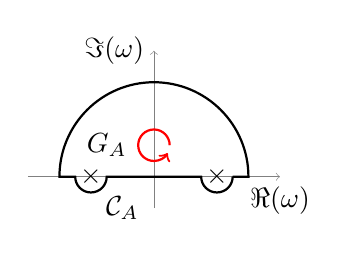
\begin{tikzpicture}[scale=0.4]
% The axes
\draw[help lines,->] (-4,0) -- (4,0) coordinate (xaxis);
\draw[help lines,->] (0,-1) -- (0,4) coordinate (yaxis);
\draw[thick,red, ->] (0.5,1) arc (0:330:0.5);
\node at (-2.0,0) {$\times$};
\node at (2.0,0) {$\times$};
\node at (-1.5,1) {$G_A$};
\node at (-1,-1) {$\mathcal{C}_A$};

\path[draw,line width=0.8pt,postaction=decorate] 
(2.5,0) -- (3,0) arc (0:180:3) -- (-2.5,0) arc (180:360:.5) -- (1.5,0) arc (180:360:.5);
            
% The labels
\node[below] at (xaxis) {$\Re(\omega)$};
\node[left] at (yaxis) {$\Im(\omega)$};
\end{tikzpicture}
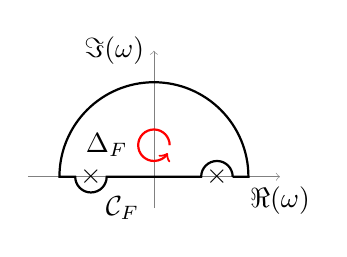
\begin{tikzpicture}[scale=0.4]
% The axes
\draw[help lines,->] (-4,0) -- (4,0) coordinate (xaxis);
\draw[help lines,->] (0,-1) -- (0,4) coordinate (yaxis);
\draw[thick,red, ->] (0.5,1) arc (0:330:0.5);
\node at (-2.0,0) {$\times$};
\node at (2.0,0) {$\times$};
\node at (-1.5,1) {$\Delta_F$};
\node at (-1,-1) {$\mathcal{C}_F$};


\path[draw,line width=0.8pt,postaction=decorate] 
(2.5,0) -- (3,0) arc (0:180:3) -- (-2.5,0) arc (180:360:.5) -- (1.5,0) arc (180:0:.5);
            
% The labels
\node[below] at (xaxis) {$\Re(\omega)$};
\node[left] at (yaxis) {$\Im(\omega)$};
\end{tikzpicture}
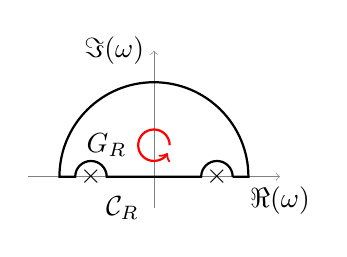
\begin{tikzpicture}[scale=0.4]
% The axes
\draw[help lines,->] (-4,0) -- (4,0) coordinate (xaxis);
\draw[help lines,->] (0,-1) -- (0,4) coordinate (yaxis);
\draw[thick,red, ->] (0.5,1) arc (0:330:0.5);
\node at (-2.0,0) {$\times$};
\node at (2.0,0) {$\times$};
\node at (-1.5,1) {$G_R$};
\node at (-1,-1) {$\mathcal{C}_R$};


\path[draw,line width=0.8pt,postaction=decorate] 
(2.5,0) -- (3,0) arc (0:180:3) -- (-2.5,0) arc (180:0:.5) -- (1.5,0) arc (180:0:.5);
            
% The labels
\node[below] at (xaxis) {$\Re(\omega)$};
\node[left] at (yaxis) {$\Im(\omega)$};
\end{tikzpicture}
\end{center}
$\tau>0$
\begin{center}
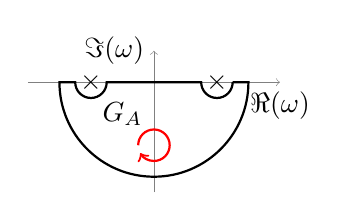
\begin{tikzpicture}[scale=0.4]
% The axes
\draw[help lines,->] (-4,0) -- (4,0) coordinate (xaxis);
\draw[help lines,->] (0,-3.5) -- (0,1) coordinate (yaxis);
\draw[thick,red, ->] (-0.5,-2) arc (180:-150:0.5);
\node at (-2.0,0) {$\times$};
\node at (2.0,0) {$\times$};
\node at (-1,-1) {$G_A$};

\path[draw,line width=0.8pt,postaction=decorate] 
(2.5,0) -- (3,0) arc (0:-180:3) -- (-2.5,0) arc (180:360:.5) -- (1.5,0) arc (180:360:.5);
            
% The labels
\node[below] at (xaxis) {$\Re(\omega)$};
\node[left] at (yaxis) {$\Im(\omega)$};
\end{tikzpicture}
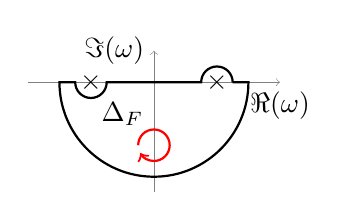
\begin{tikzpicture}[scale=0.4]
% The axes
\draw[help lines,->] (-4,0) -- (4,0) coordinate (xaxis);
\draw[help lines,->] (0,-3.5) -- (0,1) coordinate (yaxis);
\draw[thick,red, ->] (-0.5,-2) arc (180:-150:0.5);
\node at (-2.0,0) {$\times$};
\node at (2.0,0) {$\times$};
\node at (-1,-1) {$\Delta_\text{F}$};

\path[draw,line width=0.8pt,postaction=decorate] 
(2.5,0) -- (3,0) arc (0:-180:3) -- (-2.5,0) arc (180:360:.5) -- (1.5,0) arc (180:0:.5);
            
% The labels
\node[below] at (xaxis) {$\Re(\omega)$};
\node[left] at (yaxis) {$\Im(\omega)$};
\end{tikzpicture}
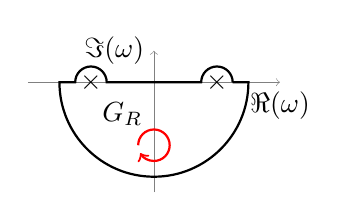
\begin{tikzpicture}[scale=0.4]
% The axes
\draw[help lines,->] (-4,0) -- (4,0) coordinate (xaxis);
\draw[help lines,->] (0,-3.5) -- (0,1) coordinate (yaxis);
\draw[thick,red, ->] (-0.5,-2) arc (180:-150:0.5);
\node at (-2.0,0) {$\times$};
\node at (2.0,0) {$\times$};
\node at (-1,-1) {$G_R$};

\path[draw,line width=0.8pt,postaction=decorate] 
(2.5,0) -- (3,0) arc (0:-180:3) -- (-2.5,0) arc (180:0:.5) -- (1.5,0) arc (180:0:.5);
            
% The labels
\node[below] at (xaxis) {$\Re(\omega)$};
\node[left] at (yaxis) {$\Im(\omega)$};
\end{tikzpicture}
\end{center}

\caption{Possible contours for the Fourier back transformation of the Greens functions of the wave equation caused by the poles $\pm ck$}
\end{figure}

\begin{enumerate}
\item Case $n=1$
\begin{align}
G(r,\tau)
&=\frac{1}{(2\pi)^2}\int dkd\omega\,\frac{c^2}{-\omega^2+c^2k^2}e^{i(kr-\omega\tau)}\\
&=\frac{1}{(2\pi)^2}\int dk\,e^{ikr}\int d\omega\,\frac{c^2}{-\omega^2+c^2k^2}e^{-i\omega\tau}\\
&=\frac{c}{2(2\pi)^2}\int dk\,\frac{e^{ikr}}{k}\int d\omega\,\left(\frac{1}{\omega+ck}-\frac{1}{\omega-ck}\right)e^{-i\omega\tau}\\
\end{align}
Now we can evaluate using the residue theorem (additional factor -1 if contour closes in mathematical negative direction)
\begin{align}
G_R(r,\tau>0)
&=\frac{c}{2(2\pi)^2}\int dk\,\frac{e^{ikr}}{k}(-1)2\pi i\left(e^{ick\tau}-e^{-ick\tau}\right)\\
&=-\frac{ic}{4\pi}\int_{-\infty}^\infty dk\,\frac{1}{k}\left(e^{ik(r+c\tau)}-e^{ik(r-c\tau)}\right)\\
&=-\frac{ic}{4\pi}\left(i\sqrt{\frac{\pi}{2}}\text{sign}(r+c\tau)-i\sqrt{\frac{\pi}{2}}\text{sign}(r-c\tau)\right)\\
&=\frac{c}{4\sqrt{2\pi}}\left(\text{sgn}(r+c\tau)-\text{sgn}(r-c\tau)\right)\\
&=\left\{\begin{matrix}
+\frac{c}{4\sqrt{2\pi}}&|z|<c\tau,& \tau>0\\
0& |z|>ct,&\\
-\frac{c}{4\sqrt{2\pi}}&|z|<c\tau,& \tau<0\\
\end{matrix}\right.\\
G_R(r,\tau<0)&=0\\
G_A(r,\tau>0)&=0\\
G_A(r,\tau<0)&=...
\end{align}

\item Case $n=2$
???

\item Case $n=3$
\begin{align}
G(\vec{r},\tau)
&=\frac{1}{(2\pi)^4}\int d^3k\;e^{i\vec{k}\vec{r}} \int d\omega\,\frac{c^2}{-\omega^2+c^2k^2}e^{-i\omega\tau}\\
&=\frac{2\pi}{(2\pi)^4}\int dk\,k^2\,d\theta\,\sin\theta\;e^{ikr\cos\theta} \int d\omega\,\frac{c^2}{-\omega^2+c^2k^2}e^{-i\omega\tau}\\
&=\frac{2\pi}{(2\pi)^4ir}\int dk\,k\,(e^{ikr}-e^{-ikr}) \int d\omega\,\frac{c^2}{-\omega^2+c^2k^2}e^{-i\omega\tau}
\end{align}
The poles at $\omega=\pm ck$ make the value of the integral not  
unique. Using the residue theorem we can evaluate the integral but the value will depend on the chosen contour - which means the Greens function is NOT unique!

Applying the wave operator to the solution we obtain 
\begin{align}
G(\vec{r},\tau)&=\frac{1}{(2\pi)^4}\int d^3k\;\int d\omega\,\frac{c^2}{-\omega^2+c^2k^2}e^{i(\vec{k}\vec{r}-\omega\tau)}\\
\Box G(\vec{r},\tau)&=\frac{1}{(2\pi)^4}\int d^3k\;\int d\omega\,e^{i(\vec{k}\vec{r}-\omega\tau)}=\delta(\vec{r})\delta(\tau)
\end{align}
where we now can integrate along any $\omega$-contour (even along the $\omega$ axis) as the poles are gone. This means the all contours give (potentially different) but valid Greens functions. The physical interpretation is that the different Greens function depend on the boundary conditions.

Now we can evaluate using the residue theorem (additional factor -1 if contour closes in mathematical negative direction)
\begin{align}
G_R(\vec{r},\tau>0)
&=\frac{c^2}{(2\pi)^3ir}\int_0^\infty dk\,k\,(e^{ikr}-e^{-ikr}) \int d\omega\,\frac{1}{-\omega^2+c^2k^2}e^{-i\omega\tau}\\
&=\frac{c}{2(2\pi)^3ir}\int_0^\infty dk\,(e^{ikr}-e^{-ikr}) \int d\omega\left(\frac{1}{\omega+ck}-\frac{1}{\omega-ck}\right)e^{-i\omega\tau}\\
&=\frac{c}{2(2\pi)^3ir}\int_0^\infty dk\,(e^{ikr}-e^{-ikr})(-1)2\pi i\left(e^{ick\tau}-e^{-ick\tau}\right)\\
&=\frac{c}{2(2\pi)^2r}\int_0^\infty dk\,(e^{ikr}-e^{-ikr})\left(e^{-ick\tau}-e^{ick\tau}\right)\\
&=\frac{c}{2(2\pi)^2r}\int_{-\infty}^\infty dk\,(e^{ik(r-c\tau)}-e^{-ik(r+c\tau)})\\
&=\frac{c}{4\pi r}\left(\delta(r-c\tau)-\delta(r+c\tau)\right)\\
&=\frac{c}{4\pi r}\delta(r-c\tau)\qquad(r,\tau>0)\\
G_R(\vec{x}-\vec{x}',t-t'>0)
&=\frac{c}{4\pi}\frac{\delta(|\vec{x}-\vec{x'}|-c(t-t'))}{|\vec{x}-\vec{x'}|}\\
G_R(\vec{x}-\vec{x}',t-t'<0)&=0\\
G_A(\vec{x}-\vec{x}',t-t'>0)&=0\\
G_A(\vec{x}-\vec{x}',t-t'<0)&=...
\end{align}
\end{enumerate}

\item Summary
\begin{align}
u(x,t)^\text{1D}_R&=
\textcolor{blue}{\frac{1}{2}\left[u_0(x+ct)+u_0(x-ct)\right]}+\frac{1}{2c}
\textcolor{red}{\int_{K^\text{1D}(x)_{ct}}u_1(\xi)d\xi}+\frac{c}{2\sqrt{2\pi}}
\textcolor{Green}{\int_\text{pLC} j(\xi,\tau)\,d\xi d\tau}\\
%
u(\vec{x},t)^\text{2D}_R&=\textcolor{red}{\frac{1}{2\pi c}\partial_t\left(\int_{K^\text{2D}(\vec{x})_{ct}} d^2\xi \frac{u_0(\vec{\xi})}{\sqrt{c^2t^2-|\vec{x}-\vec{\xi}|^2}}\right)}+\frac{1}{2\pi c}\textcolor{red}{\int_{K^\text{2D}(\vec{x})_{ct}} d^2\xi \frac{u_1(\vec{\xi})}{\sqrt{c^2t^2-|\vec{x}-\vec{\xi}|^2}}}+
\textcolor{Green}{???}\\
%
u(\vec{x},t)^\text{3D}_R&=\frac{t}{4\pi(ct)^2}\partial_t\left(t\int_{\partial K^\text{3D}(\vec{x})_{ct}}u_0(\xi)dA_\xi\right)+\frac{t}{4\pi(ct)^2}\int_{\partial K^\text{3D}(\vec{x})_{ct}}u_1(\xi)dA_\xi+\frac{c}{4\pi}
\textcolor{Green}{\int_{\partial\text{pLC}} \frac{j(\vec{\xi},\tau)}{|\vec{r}-\vec{\xi}|}\,d^3\xi d\tau}
\end{align}
\begin{figure}[!h]
$1d$\newline
\begin{center}
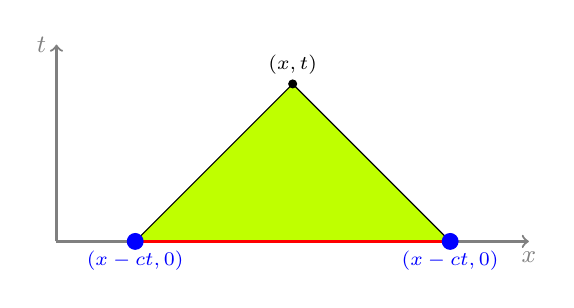
\begin{tikzpicture}
	\path [fill=lime] (4,2) -- (2,0) -- (6,0) -- (4,2);
	\draw [->, thick, gray] (1,0) -- (7,0) node [below] {\small$x$};
	\draw [->, thick, gray] (1,0) -- (1,2.5) node [left] {\small$t$};
	\draw (2,0) -- (4,2);
	\draw (4,2) -- (6,0);
	\draw [fill] (4,2) circle [radius=.05] node [above] {\scriptsize$(x,t)$};
	\draw [very thick, red] (2,0) -- (6,0);
	\draw [fill,blue] (6,0) circle [radius=.1] node [below] {\scriptsize$(x-ct,0)$};	
	\draw [fill,blue] (2,0) circle [radius=.1] node [below] {\scriptsize$(x-ct,0)$};
\end{tikzpicture}
\end{center}
\end{figure}

\end{itemize}

\newpage
\subsection{Klein-Gordon equation \texorpdfstring{$\left(\frac{1}{c^2}\partial_{tt}-\triangle+\mu^2\right) u(x,t)= j(x,t)$}{TEXT}}

\begin{itemize}
\item The free fundamental solution (no source with $j(x,t)=0$)
\begin{align}
u(\vec{x},t)&=e^{-i(k_0t-\vec{k}\vec{x})}\\
&\rightarrow\quad \frac{(-ik_0)^2}{c^2}-(i\vec{k})^2+\mu^2=0\\
&\rightarrow\quad -\frac{k_0^2}{c^2}+\vec{k}^2+\mu^2=0\\
&\rightarrow\quad k_0=\omega=\pm c\sqrt{\vec{k}^2+\mu^2}
\end{align}

\item Free solutions of
\begin{align}
\left(\frac{1}{c^2}\partial_{tt}-\triangle+\mu^2\right) u(\vec{x},t)&=0
\end{align}

\begin{align}
\varDelta(x)
&=-\int_C\frac{d^4k}{(2\pi)^4}\frac{e^{-ikx}}{k^2-\mu^2}=\frac{1}{2i}\int\frac{d^3k}{(2\pi)^3}\frac{e^{-ikx}-e^{ikx}}{\sqrt{\vec{k}^2+\mu^2}}\\
\varDelta^\pm(x)
&=-\int_{C^\pm}\frac{d^4k}{(2\pi)^4}\frac{e^{-ikx}}{k^2-\mu^2}=\mp\frac{i}{2}\int\frac{d^3k}{(2\pi)^3}\frac{e^{\mp ikx}}{\sqrt{\vec{k}^2+\mu^2}}
\end{align}

\item Sourced solution

Using
\begin{align}
\delta(\vec{x})&=\frac{1}{2\pi}\int dk e^{i\vec{k}\vec{x}}\\
G(\vec{x},t)&=\frac{1}{(2\pi)^d}\int d\vec{k}\,d\omega\,g(\vec{k},\omega)e^{i\vec{k}\vec{x}}e^{-i\omega t}
\end{align}
note the sign change of the frequency/time transform.

\begin{enumerate}
\item Case $n=1$

To find the Green function perform a 2d Fourier transform
\begin{align}
\left(\frac{1}{c^2}\partial_{tt}-\triangle+\mu^2\right) G(x-x_0,t-t_0)&= \delta(x-x_0)\delta(t-t_0)\\
\left(-\frac{\omega^2}{c^2}+k^2+\mu^2\right)\tilde{G}(k,\omega)&=1\\
\tilde{G}(k,\omega)
&=\frac{c^2}{-\omega^2+c^2(k^2+\mu^2)}\\
&=\frac{c}{2\sqrt{k^2+\mu^2}}\left(\frac{1}{\omega+c\sqrt{k^2+\mu^2}}-\frac{1}{\omega-c\sqrt{k^2+\mu^2}}\right)
\end{align}
First Fourier back transformation of $\omega$ to $t$
\begin{align}
w(k,t-t_0)&=\frac{1}{2\pi}\int d\omega\,v(\vec{k},\omega)e^{-i\omega(t-t_0)}\\
&=\frac{c}{(2\pi)2\sqrt{k^2+\mu^2}}\int_{-\infty}^{+\infty} d\omega\,e^{-i\omega(t-t_0)}\left(\frac{1}{\omega+c\sqrt{k^2+\mu^2}}-\frac{1}{\omega-c\sqrt{k^2+\mu^2}}\right)
\end{align}
we recognize the two poles at $\pm c\sqrt{k^2+\mu^2}$ on the real axis. Using the residue theorem we can decide pick four (five) contours which subsequently result in different Green functions

\begin{table}
\centering
\begin{tabular}{|l|c|c|}
\hline 
Name & Symbol & Contour \\ 
\hline 
Feynman propagator        & $\Delta_F$     & $\mathcal{C}_F$ \\
Dyson propagator          & $\Delta_D$     & $\mathcal{C}_D$ \\
Retarded propagator       & $\Delta_R$     & $\mathcal{C}_R$ \\
Advanced propagator       & $\Delta_A$     & $\mathcal{C}_A$ \\
Principle-part propagator & $\bar{\Delta}$ & $\bar{\mathcal{C}}$ \\
\hline 
\end{tabular} 
\caption{Greens functions}
\end{table}

\begin{figure}[!h]
$t-t_0<0$\newline
\begin{center}
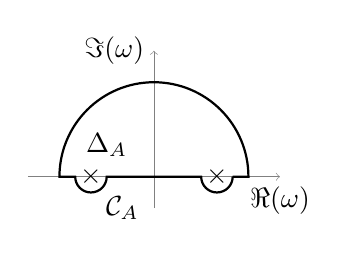
\begin{tikzpicture}[scale=0.4]
% The axes
\draw[help lines,->] (-4,0) -- (4,0) coordinate (xaxis);
\draw[help lines,->] (0,-1) -- (0,4) coordinate (yaxis);
\node at (-2.0,0) {$\times$};
\node at (2.0,0) {$\times$};
\node at (-1.5,1) {$\Delta_A$};
\node at (-1,-1) {$\mathcal{C}_A$};

\path[draw,line width=0.8pt,postaction=decorate] 
(2.5,0) -- (3,0) arc (0:180:3) -- (-2.5,0) arc (180:360:.5) -- (1.5,0) arc (180:360:.5);
            
% The labels
\node[below] at (xaxis) {$\Re(\omega)$};
\node[left] at (yaxis) {$\Im(\omega)$};
\end{tikzpicture}
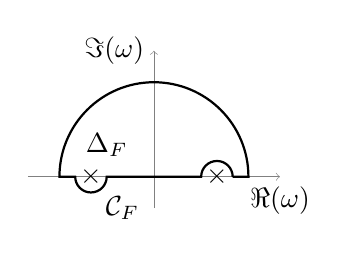
\begin{tikzpicture}[scale=0.4]
% The axes
\draw[help lines,->] (-4,0) -- (4,0) coordinate (xaxis);
\draw[help lines,->] (0,-1) -- (0,4) coordinate (yaxis);
\node at (-2.0,0) {$\times$};
\node at (2.0,0) {$\times$};
\node at (-1.5,1) {$\Delta_F$};
\node at (-1,-1) {$\mathcal{C}_F$};


\path[draw,line width=0.8pt,postaction=decorate] 
(2.5,0) -- (3,0) arc (0:180:3) -- (-2.5,0) arc (180:360:.5) -- (1.5,0) arc (180:0:.5);
            
% The labels
\node[below] at (xaxis) {$\Re(\omega)$};
\node[left] at (yaxis) {$\Im(\omega)$};
\end{tikzpicture}
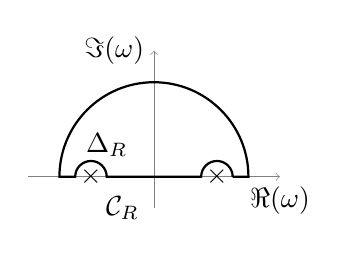
\begin{tikzpicture}[scale=0.4]
% The axes
\draw[help lines,->] (-4,0) -- (4,0) coordinate (xaxis);
\draw[help lines,->] (0,-1) -- (0,4) coordinate (yaxis);
\node at (-2.0,0) {$\times$};
\node at (2.0,0) {$\times$};
\node at (-1.5,1) {$\Delta_R$};
\node at (-1,-1) {$\mathcal{C}_R$};


\path[draw,line width=0.8pt,postaction=decorate] 
(2.5,0) -- (3,0) arc (0:180:3) -- (-2.5,0) arc (180:0:.5) -- (1.5,0) arc (180:0:.5);
            
% The labels
\node[below] at (xaxis) {$\Re(\omega)$};
\node[left] at (yaxis) {$\Im(\omega)$};
\end{tikzpicture}
\end{center}
$t-t_0>0$
\begin{center}
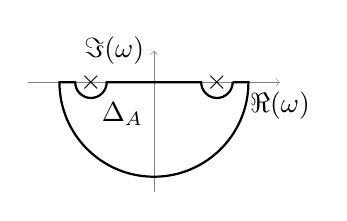
\begin{tikzpicture}[scale=0.4]
% The axes
\draw[help lines,->] (-4,0) -- (4,0) coordinate (xaxis);
\draw[help lines,->] (0,-3.5) -- (0,1) coordinate (yaxis);
\node at (-2.0,0) {$\times$};
\node at (2.0,0) {$\times$};
\node at (-1,-1) {$\Delta_A$};

\path[draw,line width=0.8pt,postaction=decorate] 
(2.5,0) -- (3,0) arc (0:-180:3) -- (-2.5,0) arc (180:360:.5) -- (1.5,0) arc (180:360:.5);
            
% The labels
\node[below] at (xaxis) {$\Re(\omega)$};
\node[left] at (yaxis) {$\Im(\omega)$};
\end{tikzpicture}
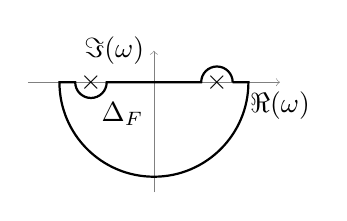
\begin{tikzpicture}[scale=0.4]
% The axes
\draw[help lines,->] (-4,0) -- (4,0) coordinate (xaxis);
\draw[help lines,->] (0,-3.5) -- (0,1) coordinate (yaxis);
\node at (-2.0,0) {$\times$};
\node at (2.0,0) {$\times$};
\node at (-1,-1) {$\Delta_\text{F}$};

\path[draw,line width=0.8pt,postaction=decorate] 
(2.5,0) -- (3,0) arc (0:-180:3) -- (-2.5,0) arc (180:360:.5) -- (1.5,0) arc (180:0:.5);
            
% The labels
\node[below] at (xaxis) {$\Re(\omega)$};
\node[left] at (yaxis) {$\Im(\omega)$};
\end{tikzpicture}
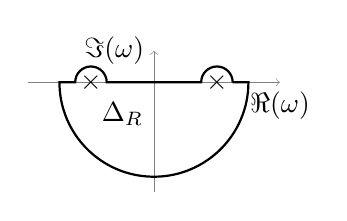
\begin{tikzpicture}[scale=0.4]
% The axes
\draw[help lines,->] (-4,0) -- (4,0) coordinate (xaxis);
\draw[help lines,->] (0,-3.5) -- (0,1) coordinate (yaxis);
\node at (-2.0,0) {$\times$};
\node at (2.0,0) {$\times$};
\node at (-1,-1) {$\Delta_R$};

\path[draw,line width=0.8pt,postaction=decorate] 
(2.5,0) -- (3,0) arc (0:-180:3) -- (-2.5,0) arc (180:0:.5) -- (1.5,0) arc (180:0:.5);
            
% The labels
\node[below] at (xaxis) {$\Re(\omega)$};
\node[left] at (yaxis) {$\Im(\omega)$};
\end{tikzpicture}
\end{center}

\caption{Possible contours for the Fourier back transformation of the one dimensional Klein-Gordon Greens functions caused by the poles $\pm c\sqrt{k^2+\mu^2}$}
\end{figure}
\begin{align}
\int_{-\infty}^\infty f\,d\omega+\int_\text{half circ} f\,d\omega=2\pi i\text{Res}f
\end{align}

$t-t_0<0:$
\begin{align}
w_A(k,t-t_0)&=\frac{2\pi i c}{4\pi\sqrt{k^2+\mu^2}}\left[e^{ic(t-t_0)\sqrt{k^2+\mu^2}}-e^{-ic(t-t_0)\sqrt{k^2+\mu^2}}\right]\\
&=\frac{-c}{\sqrt{k^2+\mu^2}}\sin\left(c(t-t_0)\sqrt{k^2+\mu^2}\right)\\
w_F(k,t-t_0)&=\frac{ic}{2\sqrt{k^2+\mu^2}}\left[-e^{-ic(t-t_0)\sqrt{k^2+\mu^2}}\right]\\
w_R(k,t-t_0)&=0
\end{align}

$t-t_0>0:$
\begin{align}
w_A(k,t-t_0)&=0\\
w_F(k,t-t_0)&=\frac{2\pi i c}{4\pi\sqrt{k^2+\mu^2}}\left[-e^{-ic(t-t_0)\sqrt{k^2+\mu^2}}\right]\\
w_R(k,t-t_0)&=\frac{2\pi i c}{4\pi\sqrt{k^2+\mu^2}}\left[e^{ic(t-t_0)\sqrt{k^2+\mu^2}}-e^{-ic(t-t_0)\sqrt{k^2+\mu^2}}\right]\\
&=\frac{-ic}{\sqrt{k^2+\mu^2}}\sin\left(c(t-t_0)\sqrt{k^2+\mu^2}\right)
\end{align}
Second Fourier back transformation
\begin{align}
u(x,t)
&=\frac{1}{2\pi}\int dk\,e^{ikx}w(k,t)\\
&=\frac{c}{4\pi^2}\int dk\frac{e^{ikx}}{\mu\sqrt{k^2/\mu^2+1}}\left[e^{-ict\mu\sqrt{k^2/\mu^2+1}}-e^{ict\mu\sqrt{k^2/\mu^2+1}}\right]
\end{align}
Now substitude $k/\mu=\sinh s$ and $1+\sinh^2s=\cosh^2s$
\begin{align}
u(x,t)
&=\frac{c}{4\pi^2}\int \mu\cosh s\,ds\frac{e^{ix\mu\sinh s}}{\mu\cosh s}\left[e^{-ict\mu\cosh s}-e^{ict\mu\cosh s}\right]\\
&=\frac{c}{4\pi^2}\int ds\,e^{ix\mu\sinh s}\left[e^{-ict\mu\cosh s}-e^{ict\mu\cosh s}\right]
\end{align}
as well as
\begin{align}
x&=\frac{1}{\mu}z\cosh y\\
ct&=\frac{1}{\mu}z\sinh y\\
&\rightarrow x^2-c^2t^2=\frac{1}{\mu^2}z^2
\end{align}
which gives
\begin{align}
u(x,t)
&=\frac{c}{4\pi^2}\int ds\,e^{iz\cosh y\sinh s}\left[e^{-iz\sinh y\cosh s}-e^{iz\sinh y\cosh s}\right]\\
&=\frac{c}{4\pi^2}\int ds\,(e^{iz(\cosh y\sinh s-\sinh y\cosh s)}-e^{iz(\cosh y\sinh s+\sinh y\cosh s)})\\
&=\frac{c}{4\pi^2}\int ds\,(e^{iz\sinh(s-y)}-e^{iz\sinh(s+y)})\\
&=\frac{c}{4\pi^2}\int ds\,\left[\cos(z\sinh(s-y))+i\sin(z\sinh(s-y))-e^{iz\sinh(s+y)}\right]
\end{align}


\begin{align}
z^2&=\mu^2(x^2-c^2t^2)\\
\psi_0(x,t)
&=\frac{i}{\pi c}\partial_t\int_0^\infty dy\,\cos(z\sinh y)\quad\text{for}\quad \psi_0(x,0)=\delta(x)\\
\psi(x,t)&=\int dy\,f(y)\psi_0(x-y,t)\quad\text{for}\quad \psi(x,0)=f(x) 
\end{align}

\item Case $n=3$

\end{enumerate}
\end{itemize}

\newpage
\subsection{Helmholtz equation \texorpdfstring{$(\triangle +k^2)u(x)= f(x)$}{TEXT}}
The Greens function is given by $(\triangle_x +k^2)G(x,y)=\delta(x-y)$

\subsection{Feynman propagator \texorpdfstring{$\left(\triangle-k^2\right) u(x)= f(x)$}{TEXT}}

\subsection{Heat equation \texorpdfstring{$\left(\partial_{t}-k\triangle\right) u(x)= f(x)$}{TEXT}}

Homogenous case $\left(\partial_{t}-k\triangle\right) G(x,t)=0$
\begin{align}
G(x,t)=\frac{1}{\sqrt{4\pi kt}}e^{-\frac{x^2}{4kt}}
\end{align}



\subsection{Relativistic Heat equation \texorpdfstring{$\left(\partial_{tt}+2\gamma\partial_t-c^2\triangle\right) u(x)= f(x)$}{TEXT}}

\subsection{Sine-Gordon equation equation \texorpdfstring{$\left(\frac{1}{c^2}\partial_{tt}-\triangle+\right) u(x,t)+\sin u(x,t)=0$}{TEXT}}

\subsection{Kortegweg-De Vries equation equation \texorpdfstring{$\partial_tu+6u\cdot\partial_x u+\partial_{xxx}u= 0$}{TEXT}}

\newpage
\section{Perturbation and divergent series}
\begin{align}
A_n&=\sum_{k=0}^{n}a_k\\
A&=\lim_{n\rightarrow\infty}A_n
\end{align}
\subsection{Shanks transform (convergence accelerators)}
For a slowly converging sum
\begin{align}
S(A_n)=\frac{A_{n+1}A_{n-1}-A_n^2}{A_{n+1}-2A_n+A_{n-1}}
\end{align}
the transformed partial sum $S(S(S(S(A_n))))$ might converge much faster than $A_n$.
\subsection{Richardson extrapolations (convergence accelerators)}
For a slowly converging sum the extrapolation
\begin{align}
R_1&=(n+1)S_{n+1}-nS_n\\
R_2&=\frac{1}{2}\left[(n+2)^2S_{n+2}-2(n+1)^S_{n+1}+n^2S_n\right]\\
R_n&=...
\end{align}

\newpage
\section{Probability}

\begin{itemize}
\item Hypothesis $H$: Steve is a librarian
\item Evidence $E$: Steve likes reading books
\end{itemize}
Question: Whats the probability of the hypothesis is true given the evidence is true $P(H|E)$ 
\begin{align}
   P(H|E)\equiv\frac{P(E\cap H)}{P(E)}\qquad P(E|H)\equiv\frac{P(E\cap H)}{P(H)}\\
   \rightarrow\qquad P(H|E)=\frac{P(E|H)\cdot P(H)}{P(E)}=\frac{P(H)\cdot P(E|H)}{P(H)\cdot P(E|H)+ P(\neg H)\cdot P(E|\neg H)}
\end{align}
alternatively
\begin{align}
  P(H|E)&=\frac{\#\text{allPeople}\cdot P(H)\cdot P(E|H)}{\#\text{allPeople}\cdot P(H)\cdot P(E|H)+\#\text{allPeople}\cdot P(\neg H)\cdot P(E|\neg H)}\\
  &=\frac{P(H)\cdot P(E|H)}{P(H)\cdot P(E|H)+ P(\neg H)\cdot P(E|\neg H)}\\
  &=\frac{P(H)\cdot P(E|H)}{P(E)}
\end{align}

\begin{center}
        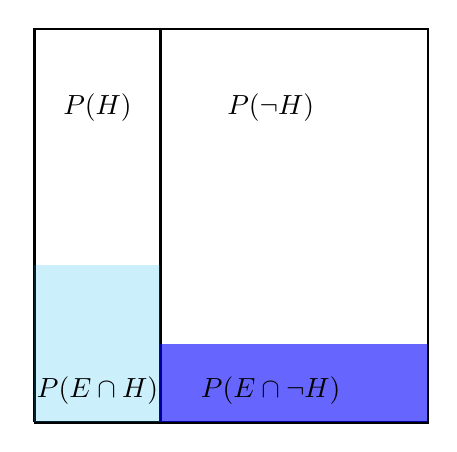
\begin{tikzpicture}
        
            \path[draw,line width=0.8pt] (0,0)  -- (5,0) -- (5,5) -- (0,5) -- (0,0);
            \path[draw,line width=0.8pt] (1.6,0)  -- (1.6,5);
            \path [fill=cyan, fill opacity=0.2] (0,0) rectangle (1.6,2);
            \path [fill=blue, fill opacity=0.6] (1.6,0) rectangle (5,1);
            
            \node at (0.8,4) {$P(H)$};
            \node at (3,4) {$P(\neg H)$};
            \node at (0.8,0.4) {$P(E\cap H)$};
            \node at (3,0.4) {$P(E\cap\neg H)$};
        \end{tikzpicture}
\end{center}


\section{Matrices}
\begin{enumerate}
    \item inverse $A^{-1}A=\mathbb{I}$
    \begin{itemize}
        \item therefore $\mathbb{I}=(AB)(B^{-1}A^{-1})\quad\rightarrow\quad (AB)^{-1}=B^{-1}A^{-1}$
    \end{itemize}
    \item Hermitian transpose $A^\dagger = (\overline{A})^T = \overline{A^T}$
        \begin{itemize}
        \item $(AB)^\dagger=B^\dagger A^\dagger$ therefore $\mathbb{I}=(AA^{-1})^\dagger=(A^{-1})^\dagger A^\dagger\quad\rightarrow\quad (A^\dagger)^{-1}=(A^{-1})^\dagger$
        \begin{align}
        \langle x |A y\rangle=\sum_k x_k^* (\vec{A}_{\text{row}k}\cdot\vec{y})=\sum_{k,l} x_k^* A_{kl}y_l\\
        \langle Bx |y\rangle = \sum_k(\vec{B}_{\text{row}k}\cdot \vec{x})^*y_k= \sum_{k,l}B_{kl}^*x_l^*y_k
        \end{align}
    \end{itemize}
    \item Real symmetric $A^T = A$
    	\begin{itemize}
    	\item only real eigenvalues
    	\item always diagonalizable
    	\end{itemize}
    \item Hermitian $A^T = \overline{A}$ or better $A^\dagger = A$
        \begin{itemize}
    	\item only real eigenvalues
    	\item always diagonalizable
    	\end{itemize}
    \item Orthorgonal $A^T = A^{-1}$
        \begin{itemize}
    	\item at most eigenvalues $\pm1$
    	\item always invertible
    	\end{itemize}
    \item Unitary $A^\dagger = A^{-1}$
    	\begin{itemize}
    	\item at most eigenvalues of from $e^{-i\alpha}$
    	\item always invertible
    	\end{itemize}
\end{enumerate}

\section{Matrix exponentials}
\begin{align}
e^X&=\sum_{n=0}\frac{1}{n!}X^n\\
\text{det}\;e^X&=e^{\text{tr} X} \\
\left(e^X\right)^{-1}&=e^{-X}\\
e^Xe^Y&=e^{X+Y+\frac{1}{2}[X,Y]+\frac{1}{12}[X,[X,Y]]-\frac{1}{12}[Y,[X,Y]]+...}
\end{align}


\section{Diagonalization}
Any  matrix $A$ is called diagonalizable if there exists an invertible matrix $S$ such that
\begin{align}
    D_A=S^{-1}AS
\end{align}
is a diagonal matrix. The diagonalizability of $A$ is equivalent to the fact that the $\{\vec{v}_i\}$ are all linearly independent. Necessary condition
\begin{itemize}
\item $n$ distinct eigenvalues
\item if there is eigenvalue with multiplicity $k$ then it must have $k$ linearly independent eigenvectors
\end{itemize}

To find $S$ and $D_A$ one has to find the eigensystem $\{\lambda_i,\vec{v}_i\}$ with $A\vec{v}_i=\lambda_i\vec{v}_i$. Then $D_AS$ and $S$ can be written as $S=(\vec{v}_1,...,\vec{v}_n)$ and $D_A=\text{diag}(\lambda_1,...,\lambda_n)$ because $AS=(A\vec{v}_1,...,A\vec{v}_n)=(\lambda_1\vec{v}_1,...,\lambda_n\vec{v}_n)=SD_A$.


\section{Functional derivatives}
Let $F[\phi]$ a functional, i.e. a mapping from a Banach space $\mathcal{M}$ to the field of real or complex numbers. The functional (Frechet) derivative $\delta F[\phi]/\delta\phi$ is defined by
\begin{align}
    \delta F
    &=\int dx \frac{\delta F[\phi]}{\delta\phi(x)}\cdot\delta\phi(x)\\
    &=\int dx \frac{\delta F[\phi]}{\delta\phi(x)}\cdot\epsilon\delta(x-y)\\
    &=\epsilon\frac{\delta F[\phi]}{\delta\phi(y)}\\
    &=F[\phi+\epsilon\delta(x-y)]-F[\phi]
\end{align}
which means
\begin{align}
    \frac{\delta F[\phi]}{\delta\phi[y]}&=\lim_{\epsilon\rightarrow0}\frac{F[\phi+\epsilon\delta(x-y)]-F[\phi]}{\epsilon}\\
    F[\phi+\epsilon\delta(x-y)]&=F[\phi]+\epsilon\frac{\delta F[\phi]}{\delta\phi(y)}\\
    &=F[\phi]+\epsilon\int dx \frac{\delta F[\phi]}{\delta\phi(x)}\cdot\delta(x-y)
\end{align}
\begin{itemize}
    \item Product rule $F[\phi]=G[\phi]H[\phi]$
    \begin{align}
        \frac{\delta F[\phi]}{\delta\phi(x)}
        &=\frac{\delta(G[\phi]H[\phi])}{\delta\phi}\\
        &=\lim_{\epsilon\rightarrow0}\frac{G[\phi+\epsilon\delta(x-y)]H[\phi+\epsilon\delta(x-y)]-G[\phi]H[\phi]}{\epsilon}\\
        &=\lim_{\epsilon\rightarrow0}\frac{\left(G[\phi]+\epsilon\frac{\delta G}{\delta\phi}\right)\left(H[\phi]+\epsilon\frac{\delta H}{\delta\phi}\right)-G[\phi]H[\phi]}{\epsilon}\\
        &=\lim_{\epsilon\rightarrow0}\frac{G[\phi]H[\phi]+\epsilon G[\phi]\frac{\delta H}{\delta\phi}+\frac{\delta G}{\delta\phi}H[\phi]+\epsilon^2\frac{\delta G}{\delta\phi}\frac{\delta H}{\delta\phi}-G[\phi]H[\phi]}{\epsilon}\\
        &=G[\phi]\frac{\delta H[\phi]}{\delta\phi(x)}+\frac{\delta G[\phi]}{\delta\phi(x)}H[\phi]
    \end{align}
    \item Chain rule $F[G[\phi]]$
    \begin{align}
        \delta F
        &=\int dx \frac{\delta F[G[\phi]]}{\delta\phi(x)} \delta\phi(x)\\
        \delta G
        &=\int dy \frac{\delta G[\phi]}{\delta\phi(y)} \delta\phi(y)\\
        \delta F
        &=\int dz \frac{\delta F[G]}{\delta G(z)} \delta G(z)\\
        &=\int dz \frac{\delta F[G]}{\delta G(z)} \int dy \frac{\delta G[\phi]}{\delta\phi(y)} \delta\phi(y) \\
        &=\int dy \underbrace{\int dz \frac{\delta F[G]}{\delta G(z)} \frac{\delta G[\phi]}{\delta\phi(y)}}_{=\frac{\delta F[G[\phi]]}{\delta\phi(y)}} \;\delta\phi(y) \\
        \frac{\delta F[G[\phi]]}{\delta\phi(y)}
        &=\int dz \frac{\delta F[G]}{\delta G(z)} \frac{\delta G[\phi]}{\delta\phi(y)}
    \end{align}
    \item Chain rule (special case) $F[g[\phi]]$
    \begin{align}
        \frac{\delta F[g[\phi]]}{\delta\phi(y)}
        &=...\\
        &=\frac{\delta F}{\delta g(\phi(y))} \frac{d g(\phi)}{d\phi(y)}
    \end{align}
\end{itemize}
Some examples
\begin{enumerate}
    \item $F[\phi]=\int dx \phi(x)\delta(x)$
    \begin{align}
        \frac{\delta F[\phi]}{\delta\phi(y)}
           &=\lim_{\epsilon\rightarrow0}\frac{1}{\epsilon}\left(\int dx(\phi(x)+\epsilon\delta(x-y))\delta(x))-\int
        dx\,\phi(x)\delta(x)\right)\\
        &=\int dx\,\delta(x-y))\delta(x)\\
       &=\delta(y)
    \end{align}
    \item $F[\phi]=\int dx \phi(x)$
    \begin{align}
        \frac{\delta F[\phi]}{\delta\phi(y)}
        &=\lim_{\epsilon\rightarrow0}\frac{1}{\epsilon}\left(\int dx(\phi(x)+\epsilon\delta(x-y)))-\int dx\,\phi(x)\right)\\
        &=\int dx\,\delta(x-y)\\
        &=1
    \end{align}
    \item $F_x[\phi]=\phi(x)$
    \begin{align}
        \frac{\delta \phi(x)}{\delta\phi(y)}=\frac{\delta F_x[\phi]}{\delta\phi(y)}
        &=\lim_{\epsilon\rightarrow0}\frac{1}{\epsilon}\left((\phi(x)+\epsilon\delta(x-y))-\phi(x)\right)\\
        &=\delta(x-y)
    \end{align}
    \item $F[\phi]=\int dx \phi(x)^n$
    \begin{align}
        \frac{\delta F[\phi]}{\delta\phi(y)}
        &=\lim_{\epsilon\rightarrow0}\frac{1}{\epsilon}\left(\int dx(\phi(x)+\epsilon\delta(x-y)))^n-\int dx\,\phi(x)^n\right)\\
        &=\int dx\,n\phi(x)^{n-1}\delta(x-y)\\
        &=n\phi(y)^{n-1}
    \end{align}
    \item $F[\phi]=\int dx \left(\frac{\phi(x)}{dx}\right)^n$
	\begin{align}
	\frac{\delta F_y[\phi]}{\delta\phi(y)}
	&=\lim_{\epsilon\rightarrow0}\frac{1}{\epsilon}\left(\int dx(\frac{d}{dx}\phi(x)+\epsilon\frac{d}{dx}\delta(x-y))^n-\int dx\,(\frac{d}{dx}\phi(x))^n\right)\\
	&=\lim_{\epsilon\rightarrow0}\frac{1}{\epsilon}\left(\int dx(\frac{d}{dx}\phi(x))^n+n(\frac{d}{dx}\phi(x))^{n-1}\epsilon\frac{d}{dx}\delta(x-y)+O(\epsilon^2)-\int dx\,(\frac{d}{dx}\phi(x))^n\right)\\
	&=\int dx\, n(\frac{d}{dx}\phi(x))^{n-1}\frac{d}{dx}\delta(x-y)\\
	&=- n\frac{d}{dx}(\frac{d}{dx}\phi(x))^{n-1}
	\end{align}	    
    
    
    \item $F_y[\phi]=\int dz K(y,z)\phi(z)$
    \begin{align}
        \frac{\delta F_y[\phi]}{\delta\phi(x)}
           &=\lim_{\epsilon\rightarrow0}\frac{1}{\epsilon}\left(\int dz(K(y,z)(\phi(z)+\epsilon\delta(z-x)) -\int dz K(y,z)\phi(z)\right)\\
           &=\int dz\,K(y,z)\delta(z-x)\\
           &=K(y,x)
    \end{align}
    \item $F_x[\phi]=\nabla\phi(x)$
    \begin{align}
        \frac{\delta F[\phi]}{\delta\phi(y)}
        &=\lim_{\epsilon\rightarrow0}\frac{1}{\epsilon}\left( \nabla_x(\phi(x)+\epsilon\delta(x-y)) - \nabla_x\phi(x)\right)\\
        &=\nabla_x\delta(x-y)
    \end{align}
    \item $F[\phi]=g\left(G[\phi(x)]\right)$
    \begin{align}
        \frac{\delta F[\phi]}{\delta\phi(y)}
        &=\lim_{\epsilon\rightarrow0}\frac{1}{\epsilon}g(G[\phi(x)+\epsilon\delta(x-y)])-g(G[\phi(x)])\\
        &=\lim_{\epsilon\rightarrow0}\frac{1}{\epsilon}g(G[\phi(x)]+\epsilon\frac{\delta G}{\delta \phi})-g(G[\phi(x)])\\
        &=\lim_{\epsilon\rightarrow0}\frac{1}{\epsilon}g(G[\phi(x)])+g' \epsilon\frac{\delta G}{\delta \phi}-g(G[\phi(x)])\\
        &=\frac{\delta G}{\delta \phi}g'(G[\phi(x)])
    \end{align}
    
\end{enumerate}

\section{Complex Calculus}
\begin{itemize}
\item Cauchy–Riemann equations $f(x+iy)=u(x,y)+iv(x,y)$
\begin{align}
\frac{\partial u}{\partial x}&=\frac{\partial v}{\partial y}\\
\frac{\partial u}{\partial y}&=-\frac{\partial v}{\partial x}
\end{align}
\item Cauchy integral formula
\begin{align}
f(a)&=\frac{1}{2\pi i}\oint_C\frac{f(z)}{z-a}dz\\
f^{(n)}(a)&=\frac{n!}{2\pi i}\oint_C\frac{f(z)}{(z-a)^{n+1}}dz
\end{align}
\item Taylor series
\begin{align}
f(a+h)
&=\frac{1}{2\pi i}\oint_C\frac{f(z)}{z-a-h}dz\\
&=\frac{1}{2\pi i}\oint_C\frac{f(z)}{z-a}\frac{1}{1-\frac{h}{z-a}}dz\\
&=\frac{1}{2\pi i}\oint_C\frac{f(z)}{z-a}\sum_k\frac{h^k}{(z-a)^k}dz\qquad\text{(geometric series)}\\
&=\sum_k \frac{1}{2\pi i}\oint_C\frac{f(z)}{(z-a)^{k+1}}dz\cdot h^k\qquad\text{(quick and dirty - exchanging integral and sum)}\\
&=\sum_k \frac{f^{(k)}(a)}{k!}\; h^k
\end{align}

\end{itemize}

\section{Space hierarchy}
\begin{enumerate}
    \item K-Vector space $(K,\oplus,\odot)$ 
        \begin{itemize}
            \item set $V$, field $K$ with $(K,+,\cdot)$
            \item vector addition $\oplus: V\times V\rightarrow V$
            \item scalar multiplication $\odot: K\times V\rightarrow V$
        \end{itemize}
    \item Topological vector space
        \begin{itemize}
            \item K-vector space
            \item continuous (smooth) vector addition and scalar multiplication
        \end{itemize}
    \item Metric (vector) space $(M,d)$
        \begin{itemize}
            \item set $M$, metric $d: M\times M\rightarrow \mathbb{R}$
            \item $d(x,y)=0 \Leftrightarrow x=y$
            \item $d(x,y)=d(y,x)$
            \item $d(x,y)+d(y,z) \ge d(x,z)$
            \item from the requirements above follows $d(x,y)\ge0$
        \end{itemize}
    \item Normed vector space $(V,\|\cdot\|)$
        \begin{itemize}
            \item K-vector space $V$, norm $\|\cdot\|: V\rightarrow \mathbb{R}$
            \item Typically $K\in(\mathbb{R}, \mathbb{C})$ to have a definition of $|\lambda|$
            \item $\|x\|\ge0$
            \item $\|x\|=0 \Leftrightarrow x=0$
            \item $\|\lambda x\|=|\lambda| \|x\|$ with $\lambda\in K$
            \item $\|x\|+\|y\|\ge\|x+y\|$
            \item with $d(x,y):=\|x-y\|$ every normed vector space has also a metric
            \item a metric does NOT induce a always norm as the linearity/homogeneity of the norm is not guaranteed 
        \end{itemize}
    \item Banach space (complete normed vector space)
        \begin{itemize}
            \item normed K-vector space $(V,\|\cdot\|)$ with $K\in(\mathbb{R}, \mathbb{C})$
            \item completeness: every Cauchy sequence converges (with the metric induced by the norm) to a well defined limit
            \item if the space is just a metric space (without a norm) the space is called Cauchy space
        \end{itemize}
    \item Hilbert space (complete vector space with a scalar product)
        \begin{itemize}
            \item K-vector space $V$ with $K\in(\mathbb{R}, \mathbb{C})$
            \item scalar product $\langle\cdot,\cdot\rangle:V\times V\rightarrow K$
            \item $\langle \lambda x_1+x_2,y\rangle = \langle \lambda x_1,y\rangle + \langle \lambda x_2,y\rangle$
            \item $\langle \lambda x,y\rangle = \lambda\langle x,y\rangle$ for $\lambda\in K$
            \item $\langle x,y\rangle=\overline{\langle y,x\rangle}$ which implies $\langle x,x\rangle \in \mathbb{R}$
            \item $\langle x,x\rangle>0$
            \item $\langle x,x\rangle=0\Leftrightarrow x=0$
            \item completeness: every Cauchy sequence converges (with the metric induced by the norm which is itself induced by the scalar product) to a well defined limit
            \item without completeness the space is called Pre-Hilbert space
        \end{itemize}
\end{enumerate}

\section{Tensors}
\begin{itemize}
\item For a vector $\mathbf{A}$ the expression $\mathbf{A}^2$ is the squared distance between tip and tail.
\item The inner product of two vectors can then be defined by the parallelogram law
\begin{align}
    \mathbf{A}\cdot\mathbf{B}\equiv\frac{1}{4}\left[(\mathbf{A}+\mathbf{B})^2-(\mathbf{A}-\mathbf{B})^2\right]
\end{align}
\item A rank-$n$ tensor $\mathbf{T}=\mathbf{T}(\_,\_,\_)$ is real-valued linear function of $n$ vectors.
\begin{align}
    \mathbf{T}(\alpha\mathbf{A}+\mu\mathbf{B},\mathbf{C},\mathbf{D})=\alpha\mathbf{T}(\mathbf{A},\mathbf{C},\mathbf{D})+\beta\mathbf{T}(\mathbf{B},\mathbf{C},\mathbf{D})
\end{align}
\item Metric tensor
\begin{align}
    \mathbf{g}(\mathbf{A},\mathbf{B})\equiv\mathbf{A}\cdot\mathbf{B}
\end{align}
\item A vector is a tensor of rank one 
\begin{align}
    \mathbf{A}(\mathbf{C})\equiv\mathbf{A}\cdot\mathbf{C}
\end{align}
\item Tensor product 
\begin{align}
    \mathbf{A}\otimes\mathbf{B}\otimes\mathbf{C}(\mathbf{E},\mathbf{F},\mathbf{G})\equiv\mathbf{A}(\mathbf{E})\mathbf{B}(\mathbf{F})\mathbf{C}(\mathbf{G})=(\mathbf{A}\cdot\mathbf{E})(\mathbf{B}\cdot\mathbf{F})(\mathbf{C}\cdot\mathbf{G})
\end{align}
\item Contraction
\begin{align}
    \text{1\&3 contraction}(\mathbf{A}\otimes\mathbf{B}\otimes\mathbf{C}\otimes\mathbf{D})\equiv(\mathbf{A}\cdot\mathbf{C})\mathbf{B}\otimes\mathbf{D}
\end{align}
\item Orthogonal basis
\begin{align}
    \mathbf{e}_j\cdot\mathbf{e}_k=\delta_{jk}
\end{align}
\item Component expansion
\begin{align}
    \mathbf{A}=A_j\mathbf{e}_j\quad&\rightarrow\quad A_j=\mathbf{A}(\mathbf{e}_j)=\mathbf{A}\cdot\mathbf{e}_j\\
    \mathbf{T}=T_{abc}\mathbf{e}_a\otimes\mathbf{e}_b\otimes\mathbf{e}_c\quad&\rightarrow\quad T_{ijk}=\mathbf{T}(\mathbf{e}_i,\mathbf{e}_j,\mathbf{e}_k)\\
    \text{1\&3 contraction}(\mathbf{R})\quad&\rightarrow\quad R_{ijik}\\
    \mathbf{g}\quad&\rightarrow\quad g_{jk}=\mathbf{g}(\mathbf{e}_j,\mathbf{e}_k)=\mathbf{e}_j\cdot\mathbf{e}_k=\delta_{jk}
\end{align}
\end{itemize}

\section{Tensors Index rules}
$A_{ij}$ - $i$-th row and $j$-th column
\begin{align}
C&=AB\\
C_{ij}&=\sum_kA_{ik}C_{kj}
\end{align}
Matrix - Vector
\begin{align}
\Lambda\mathbf{a}\rightarrow \Lambda^i_{\;j}a^j
\end{align}
Vector - Vector
\begin{align}
\mathbf{a}\cdot\mathbf{b}&\equiv G(\mathbf{a},\mathbf{b})\\
&=G(\sum_i a^i\mathbf{e}_i,\sum_j b^j\mathbf{e}_j)\\
&=\sum_{ij}a^ib^jG(\mathbf{e}_i,\mathbf{e}_j)\\
&=\sum_{ij}a^ib^jg_{ij}\\
&=a^i g_{ij} b^j\quad=\mathbf{a}^T\;G\;\mathbf{b}\\
&=a_i b^i
\end{align}
Matrix - Matrix
\begin{align}
\eta_{\alpha\beta}dx^\alpha dx^\beta&=\eta_{\mu\nu}(\Lambda^\mu_{\;\alpha}dx^\alpha)(\Lambda^\nu_{\;\beta}dx^\beta)\\
\mathbf{dx}^T\eta\mathbf{dx}&=(\Lambda\mathbf{dx})^T\eta\Lambda \mathbf{dx}=\mathbf{dx}^T(\Lambda^T\eta\Lambda)\mathbf{dx}\\
\eta&=\Lambda^T\eta\Lambda\\
\eta_{\alpha\beta}&=\Lambda^\mu_{\;\alpha}\eta_{\mu\nu}\Lambda^\nu_{\;\beta}
\end{align}

\begin{align}
F^{ab}=\Lambda^a_{\,c}\Lambda^b_{\,d} F^{cd}\qquad\rightarrow\Lambda F\Lambda^T\\
F_{ab}=\Lambda^c_{\,a}\Lambda^d_{\,b} F_{cd}\qquad\rightarrow\Lambda^T F\Lambda
\end{align}

\begin{align}
F^a_{\;b}&=\eta^{ac}F_{cb}\qquad\rightarrow \eta F\\
F^{ad}&=\eta^{db}\eta^{ac}F_{cb}=\eta^{ac}F_{cb}\eta^{bd}\qquad\rightarrow \eta F\eta^T\\
F_{ab}F^{ab}&=-F_{ba}F^{ab}\qquad\rightarrow-\text{tr}(F F)
\end{align}

\section{Direct Sum and Tensor Products}
Two vector spaces $V, W$ with $\dim V=n$, $\dim W=m$ and with bases
\begin{align}
\vec{e}_1=\left(\begin{array}{c}
1\\
0
\end{array}\right),\qquad
\vec{e}_2=\left(\begin{array}{c}
0\\
1
\end{array}\right)\qquad\in V
\end{align}
\begin{align}
\vec{f}_1=\left(\begin{array}{c}
1\\
0\\
0
\end{array}\right),\qquad
\vec{f}_2=\left(\begin{array}{c}
0\\
1\\
0
\end{array}\right)\qquad
\vec{f}_3=\left(\begin{array}{c}
0\\
0\\
1
\end{array}\right)\qquad\in W
\end{align}
\subsection{Direct sum}
Then
\begin{align}
\vec{v}\oplus\vec{w}
=\left(\begin{array}{c}
\vec{v}\\
\vec{w}
\end{array}\right)
\end{align}
and therefore (counting basis vectors) $\dim{V\oplus W}=n+m$. Linear maps (via matrices) can be written as
\begin{align}
(\textcolor{blue}{A}\oplus \textcolor{red}{B})
(\textcolor{blue}{\vec{v}}\oplus\textcolor{red}{\vec{w}})=
\left(\begin{array}{cc}
\textcolor{blue}{A} & 0_{n\times m}\\
0_{n\times m} & \textcolor{red}{B}\\
\end{array}\right)
\left(\begin{array}{c}
\textcolor{blue}{\vec{v}}\\
\textcolor{red}{\vec{w}}
\end{array}\right)
=(A\vec{v})\oplus(B\vec{w})
\end{align}
and also
\begin{align}
\det(A\oplus B)&=(\det A)(\det B)\\
\text{tr}(A\oplus B)&=(\text{tr} A)+(\text{tr} B)
\end{align}
\subsection{Tensor product}
Then
\begin{align}
\vec{v}\otimes\vec{w}
&=(\sum_i v^i\vec{e}_i)\otimes(\sum_j w^j\vec{f}_j)\\
&=\sum_{i,j} v^iw^j (\vec{e}_i\otimes\vec{f}_j)
\end{align}
and therefore (counting basis vectors $\vec{e}_i\otimes\vec{f}_j$) $\dim{V\otimes W}=n\cdot m$. The basis vectors can be written explicitly (stacking $n$ zero vectors $\vec{0}_m$ on top of each other)
\begin{align}
\vec{b}_k
&=\vec{e}_i\otimes\vec{f}_j\\
&=\left(\begin{array}{l}
\vec{0}_m\\ \hline
...\\ \hline
0\\
...\\
1 \quad(i^\text{th} \text{ slot } j^\text{th} \text{position})\\ 
...\\
0\\ \hline
...\\ \hline
\vec{0}_m
\end{array}\right)
\qquad\rightarrow\qquad
\vec{v}\otimes\vec{w}
=\left(\begin{array}{l}
v^1w^1\\
v^1w^2\\
v^1w^3\\ \hline
v^2w^1\\
v^2w^2\\
v^2w^3\\
\end{array}\right)
\end{align}
Alternatively visualise it as
\begin{align}
\vec{v}\otimes\vec{w}
=\vec{v}\vec{w}^\dagger
=\left(\begin{matrix}
v^1\\v^2
\end{matrix}\right)
(w^1\,w^2\,w^3)
=\left(\begin{matrix}
v^1w^1 & v^1w^2 & v^1w^3 \\
v^2w^1 & v^2w^2 & v^2w^3
\end{matrix}\right)
\end{align}
Linear maps (via matrices) can be written as
\begin{align}
\textcolor{red}{(A\otimes B)}
\textcolor{blue}{(\vec{v}\otimes\vec{w})}=
\textcolor{red}{
\left(\begin{array}{ccc}
a_{11} B & ... & a_{1n}B\\
...      & ... & ...\\
a_{n1} B & ... & a_{nn}B\\
\end{array}\right)}
\textcolor{blue}{
\left(\begin{array}{c}
v_1\vec{w}\\
...\\
v_n \vec{w}
\end{array}\right)}
=(A\vec{v})\otimes(B\vec{w})
\end{align}
Be careful with sloppy notation for addition of operators - $A+B$ is not defined on $V$ or $W$ but CAN be defined on $V\otimes W$ via
\begin{align}
A+B\equiv A\otimes I_{m\times m} + I_{n\times n}\otimes B
\end{align}
and also
\begin{align}
\det(A\otimes B)&=(\det A)^m(\det B)^n\\
\text{tr}(A\otimes B)&=(\text{tr} A)\cdot(\text{tr} B)
\end{align}


\section{Clebsch-Gordon decomposition in QM}
Falling from the sky
\begin{align}
\mathcal{H}_{j_1}\otimes\mathcal{H}_{j_2}
=\mathcal{H}_{|j_1-j_2|}\oplus...\oplus\mathcal{H}_{j_1+j_2}
\end{align}
Using the notation 
\begin{center}
\begin{tabular}{cccc}
$\mathcal{H}_{j_1}$ & $\dim{\mathcal{H}_{j_1}}$ & $\mathbf{2j_1+1}$ & Multiplett\\ \hline
$\mathcal{H}_{0}$ & $0$ & $\mathbf{0}$ & Singlet\\
$\mathcal{H}_{1/2}$ & $2$ & $\mathbf{2}$ & Doublet\\
$\mathcal{H}_{1}$ & $3$ & $\mathbf{3}$ & Triplett\\
$\mathcal{H}_{3/2}$ & $4$ & $\mathbf{4}$ & Quartett
\end{tabular}
\end{center}
Examples
\begin{align}
j_1=\frac{1}{2}, j_2=\frac{1}{2}\quad&\rightarrow\quad\mathbf{2}\otimes\mathbf{2}=\mathbf{1}\oplus\mathbf{3}
\quad\rightarrow\quad \text{1 singlet, 1 triplett}\\
j_1=1, j_2=1\quad&\rightarrow\quad\mathbf{3}\otimes\mathbf{3}=\mathbf{1}\oplus\mathbf{3}\oplus\mathbf{5}
\quad\rightarrow\quad \text{1 singlet, 1 triplett, 1 quintett}
\end{align}
Extension to three angular momentum
\begin{align}
\mathcal{H}_{j_1}\otimes\mathcal{H}_{j_2}\otimes\mathcal{H}_{j_3}
=(\mathcal{H}_{j_1}\otimes\mathcal{H}_{j_2})\otimes\mathcal{H}_{j_3}
=(\mathcal{H}_{|j_1-j_2|}\otimes\mathcal{H}_{j_3})\oplus...\oplus(\mathcal{H}_{j_1+j_2}\otimes\mathcal{H}_{j_3})
\end{align}
then
\begin{align}
j_1=1, j_2=1, j_3=1\quad
&\rightarrow(\mathcal{H}_1\otimes\mathcal{H}_1)\otimes\mathcal{H}_1=(\mathcal{H}_0\oplus\mathcal{H}_1\oplus\mathcal{H}_2)\otimes\mathcal{H}_1\\
&\qquad\qquad\qquad\qquad\quad=(\mathcal{H}_0\otimes\mathcal{H}_1)\oplus(\mathcal{H}_1\otimes\mathcal{H}_1)\oplus(\mathcal{H}_2\otimes\mathcal{H}_1)\\
&\qquad\qquad\qquad\qquad\quad=(\mathcal{H}_1)\oplus(\mathcal{H}_0\oplus\mathcal{H}_1\oplus\mathcal{H}_2)\oplus(\mathcal{H}_1\oplus\mathcal{H}_2\oplus\mathcal{H}_3)\\
&\rightarrow\mathbf{3}\otimes\mathbf{3}\otimes\mathbf{3}=\mathbf{1}\oplus\mathbf{3}\oplus\mathbf{3}\oplus\mathbf{3}\oplus\mathbf{5}\oplus\mathbf{5}\oplus\mathbf{7}
\quad\rightarrow\quad  ...
\end{align}


\section{Tensorproduct in QM}
Given two Hilbert spaces $\mathcal{V}_1, \mathcal{V}_2$ with complete orthonormal basis $\{|u_{i\in I}\rangle\}$ and $\{|v_{k\in K}\rangle\}$. The tensor product of two states $|\psi\rangle\in\mathcal{V}_1, |\phi\rangle\in\mathcal{V}_2$
is defined by
\begin{align}
|\psi\rangle_1 \otimes |\phi\rangle_2= |\phi\rangle_2 \otimes |\psi\rangle_1\in \mathcal{V}
\end{align}
with linearity restrictions
\begin{align}
a(|\psi\rangle_1 \otimes |\phi\rangle_2)
&=(a|\psi\rangle_1) \otimes |\phi\rangle_2
=|\psi\rangle_1 \otimes (a|\phi\rangle_2)\\
(|\psi_1\rangle_1 + |\psi_2\rangle_1)\otimes|\phi\rangle_2
&=|\psi_1\rangle_1\otimes|\phi\rangle_2 + |\psi_2\rangle_1\otimes|\phi\rangle_2
\end{align}
Combining two basis vectors from each of the two Hilbert spaces gives as basis of $\mathcal{V}$
\begin{align}
\{|u_i\rangle_1\otimes|v_j\rangle_2\}
\end{align}
meaning that $\dim \mathcal{V}=\dim \mathcal{V}_1\cdot\dim \mathcal{V}_2$.
Therefore each element of $\mathcal{V}$ can be represented by
\begin{align}
|\chi\rangle=\sum_{ij}a_{ij}(|u_i\rangle_1\otimes|v_j\rangle_2)
\end{align}
while the tensor product of two states is
\begin{align}
|\psi\rangle_1 \otimes |\phi\rangle_2
&=\left(\sum_ic_i|u_i\rangle\right)\otimes\left(\sum_id_i|v_i\rangle\right)\\
&=\sum_{ij}c_id_j(|u_i\rangle_1\otimes|v_j\rangle_2)
\end{align}
{\bf Question:} Can every state in $\mathcal{V}$ be expressed as a tensor product of two states in $\mathcal{V}_1$ and $\mathcal{V}_2$? {\bf Answer:} No!  (simple counter example). States which can not be  written as a product are called \underline{entangled  states}.

The scalar product of $\mathcal{V}$ space can be defined by
\begin{align}
{}_1\langle\psi|\otimes{}_2\langle\phi|)
(|\psi'\rangle_1\otimes|\phi'\rangle_2)=
{}_1\langle\psi|\psi'\rangle_1\,{}_2\langle\phi|\phi'\rangle_2
\end{align}
With orthonormal basis $\{u\}\in\mathcal{V}_1$ and $\{v\}\in\mathcal{V}_2$
\begin{align}
\langle u_i|u_k\rangle&=\delta_{ik}\\
\langle v_j|v_l\rangle&=\delta_{jl}
\end{align}
then
\begin{align}
{}_1\langle u_i|\otimes{}_2\langle v_j|)
(|u_k\rangle_1\otimes|v_l\rangle_2)=
{}_1\langle u_i|u_k\rangle_1\,{}_2\langle v_j|v_l\rangle_2=\delta_{ik}\delta_{jl}
\end{align}
meaning the basis of $\mathcal{V}$ is also orthonormal.

Operators $A$ and $B$ defined on Hilbert spaces $\mathcal{V}_1$ and $\mathcal{V}_2$ can be promoted to operators on $\mathcal{V}$ by
\begin{align}
A&\rightarrow A\otimes 1_B\\
B&\rightarrow 1_A\otimes B\\
A+B&\equiv A\otimes 1_B + 1_A\otimes B
\end{align}
then
\begin{align}
(A \otimes B)|\chi\rangle 
&:=(A|\phi\rangle_1)\otimes (B|\phi\rangle_2)\\
&=\sum_{ij}a_{ij}(A\otimes B) (|u_j\rangle_1)\otimes |v_j\rangle_2)\\
&=\sum_{ij}a_{ij} (A|u_j\rangle_1)\otimes (B|v_j\rangle_2)
\end{align}
or
\begin{align}
(A \otimes B)(|\phi\rangle_1\otimes|\phi\rangle_2) 
:=(A|\phi\rangle_1)\otimes (B|\phi\rangle_2)\\
=\sum_{ij}c_id_j(A| u_j\rangle_1)\otimes (B|v_j\rangle_2)
\end{align}
with eigenvectors $A|\phi_a\rangle=a|\phi_a\rangle$ and $B|\phi_b\rangle=b|\phi_b\rangle$
\begin{align}
(A + B)(|\phi_a\rangle\otimes|\phi_b\rangle)=...
=(a+b) |\phi_a\rangle\otimes |\phi_b\rangle
\end{align}
Examples
\begin{align}
\mathbb{R}^3\otimes\mathbb{R}^3&\simeq\mathbb{R}^9\\
\mathbb{R}\otimes\mathbb{R}\otimes\mathbb{R}&\simeq\mathbb{R}\\
\mathbb{R}\oplus\mathbb{R}\oplus\mathbb{R}&\simeq\mathbb{R}^3
\end{align}



\section{Pauli Matrices}
Properties of the Pauli matrices
\begin{align}
\sigma_1=\left(
\begin{matrix}
0    & 1\\
1 &  0
\end{matrix}
\right)\qquad
\sigma_2=\left(
\begin{matrix}
0    & -i\\
i &  0
\end{matrix}
\right)\qquad
\sigma_3=
\left(
\begin{matrix}
1 & 0\\
1 &  -1
\end{matrix}
\right)\\
%
\left[\frac{\sigma_i}{2},\frac{\sigma_j}{2}\right]=i\epsilon_{ijk}\frac{\sigma_k}{2}\qquad\left\{\sigma_i,\sigma_j\right\}=2\delta_{ij}\\
\mathrm{Tr}\sigma_i=0\qquad\mathrm{Tr}(\sigma_i\sigma_j)=2\delta_{ij}\\
\sigma_i\sigma_j=\delta_{ij}+i\epsilon_{ijk}\sigma_k\qquad\sigma_i^2=1\\
\sum_i(\sigma_i)_{ab}(\sigma_i)_{cd}=2(\delta_{bc}\delta_{ad}-\frac{1}{2}\delta_{ab}\delta_{cd})
\end{align}
The fundamental representation of SU(2) is given by $2\times2$ matrices $U$ (with $U^\dagger U=1$ and $\det U=1$) which operate on two-component column vectors (fundamental doublet or Pauli spinor) $\xi'=U\xi$. A general matrix $U$ can be expressed as
\begin{align}
U=e^{\frac{i}{2}\theta_i\sigma_i}.
\end{align}


\section{Division Algebras}
There are exactly four real division algebras with an identity element
\begin{itemize}
\item $\mathbb{R}=\{1\}$ (dimension 1)
\item $\mathbb{C}=\{1,i\}$ (dimension 2) with $i^2=-1$
\item $\mathbb{H}=\{1,i_1,i_2,i_3\}$  (dimension 4) with $i_1^2=i_2^2=i_3^2=-1$
\item $\mathbb{O}=\{1,i_1,...,i_7\}$ (dimension 8) with $i_k^2=-1$
\end{itemize}
where the $i_k$ obey
\begin{align}
i_k\circ i_l + i_l\circ i_k = 2\delta_{kl}
\end{align}
This can be generalized to a Clifford algebra by
\begin{align}
i_k\circ i_l + i_l\circ i_k = 2\sigma_k\delta_{kl}
\end{align}
where $\sigma_k=\pm1$. If $\sigma_1=...=\sigma_p=-1$ and $\sigma_{p+1}=...=\sigma_q=+1$ it is called Cl($p,q,\mathbb{R}$). Some examples are:
\begin{itemize}
\item $\text{Cl}(1,0,\mathbb{R})\cong\mathbb{C}$
\item $\text{Cl}(2,0,\mathbb{R})\cong\mathbb{H}$
\item $\text{Cl}(3,1,\mathbb{R})\rightarrow$ spin 1/2
\end{itemize}




\section{Clifford Algebras}
Cliff($1,d-1$) is defined as set of $d$ matrices of shape $n\times n$
\begin{align}
\{(\gamma^\mu)^A_{\;B}\}_{\mu\in\{0,1,...,d-1\}}\qquad A,B=1,...,n
\end{align}
which obey
\begin{align}
\left\{\gamma^\mu,\gamma^\nu\right\}\equiv\gamma^\mu\gamma^\nu+\gamma^\nu\gamma^\mu&=2\eta^{\mu\nu}\mathbf{1}_{n\times n}\\
(\gamma^\mu)^A_{\;B}(\gamma^\nu)^B_{\;C}+(\gamma^\nu)^A_{\;B}(\gamma^\mu)^B_{\;C}&=2\eta^{\mu\nu}(\mathbf{1}_{n\times n})^A_{\;C}
\end{align}
with spinor indices $A, B$ and space-time indices $\mu, \nu$.

Some properties of Clifford algebras
\begin{itemize}
\item With $\text{diag}\,\eta^{\mu\nu}=(1,-1,-1,-1)$
\begin{align}
(\gamma^0)^2=\mathbf{1}_{n\times n}\qquad(\gamma^i)^2=-\mathbf{1}_{n\times n}
\end{align}
\item The irreducible representations of Cliff($1,d-1$) have dimensions
\begin{itemize}
\item $d$ even: $n=2^{d/2}$
\item $d$ odd: $n=2^{(d-1)/2}$
\end{itemize}

\begin{center}
\begin{table}[h]
\centering
\begin{tabular}{|c|c|c|c|c|c|}
\hline
$d$ & 1            & 2            & 3            & 4            & 5, 6, 7, 8\\ \hline\hline
algebra    & Cliff($1,0$) & Cliff($1,1$) & Cliff($1,2$) &   Cliff($1,3$) & Cliff($1,d-1$)\\ \hline
$n$ & 1            & 2            & 2            & 4            & 
4, 8, 8, 16\\ \hline
\end{tabular}
\caption{•}
\end{table}
\end{center}

\item The $d$ matrices $\{\gamma^\mu\}$ of the Clifford algebra Cliff($1,d-1$) induce $d(d-1)/2$ matrices $S^{\rho\sigma}$  
\begin{align}
(S^{\rho\sigma})^A_{\;B}=\frac{i}{4}[\gamma^\rho,\gamma^\sigma]^A_{\;B}
\end{align}
which form a representation of the Lie algebra (of the Lorentz group) $\mathfrak{so}(1,d-1)$.

\item For $d=4$ we have Cliff(1,3) which contains $1+(d-1)=4$ matrices of shape $4\times4$
\begin{align}
\gamma^0, \gamma^1, \gamma^2, \gamma^3
\end{align}
which induces 6 matrices $S^{01}, S^{12}, S^{23}, S^{02}, S^{03}, S^{13}$ which are the generators of $\mathfrak{so}(1,3)$.

\item Chiral/Dirac representation of Cliff(1,3)
\begin{align}
\gamma^0=\left(\begin{matrix}
0 & \mathbf{1}_{2\times2}\\
\mathbf{1}_{2\times2} & 0
\end{matrix}\right),\qquad
\gamma^i=\left(\begin{matrix}
0 & \sigma^i\\
-\sigma^i & 0
\end{matrix}\right)
\end{align}
The $\gamma$'s act on a complex vector space - the space of Dirac spinors $(\gamma^\mu)^A_{\;B}\psi^B$. A Lorentz trafo look like
\begin{align}
\psi^A(x)&\rightarrow\left[e^{-i\omega_{\rho\sigma}S^{\rho\sigma}}\right]^A_{\;B}\psi^B(x)\\
&=\left[e^{-i(\omega_{01}S^{01}+...+\omega_{23}S^{23})}\right]^A_{\;B}\psi^B(x)\\
&=\left[e^{\frac{1}{4}(\omega_{01}[\gamma^0,\gamma^1]+...+\omega_{23}[\gamma^2,\gamma^3])}\right]^A_{\;B}\psi^B(x)
\end{align}

\end{itemize}

\section{Spinors}
3D vector ($x,y,z\in\mathbb{R}$) can be written as a Pauli vector (via the Pauli matrices) which can be written as a product of Pauli spinors ($\xi_1,\xi_2\in\mathbb{C}$) 
\begin{align}
\vec{v}=
\left(
\begin{matrix}
x\\
y\\
z
\end{matrix}
\right)
\Longleftrightarrow
x\sigma_x+y\sigma_y+z\sigma_z
&=\vec{v}\cdot\vec{\sigma}\\
&=x\left(
\begin{matrix}
0    & 1\\
1 &  0
\end{matrix}
\right)+
y\left(
\begin{matrix}
0    & -i\\
i &  0
\end{matrix}
\right)+
z\left(
\begin{matrix}
1 & 0\\
1 &  -1
\end{matrix}
\right)\\
&=\left(
\begin{matrix}
z    & x-yi\\
x+yi &  -z
\end{matrix}
\right)\\
&=\left(
\begin{matrix}
-\xi_1\xi_2 & \xi_1^2\\
-\xi_2^2    & \xi_1\xi_2
\end{matrix}
\right)\\
&=\left(
\begin{matrix}
\xi_1 \\
\xi_2 
\end{matrix}
\right)
\left(
\begin{matrix}
-\xi_2&\xi_1 
\end{matrix}
\right)
\end{align}
Rotating a vector
\begin{align}
\left(
\begin{matrix}
1 & 0 & 0\\
0 & \cos\theta & -\sin\theta\\
0 & \sin\theta & \cos\theta\\
\end{matrix}
\right)\left(
\begin{matrix}
x\\
y\\
z
\end{matrix}
\right)
\end{align}
Rotating the associated Pauli vector
\begin{align}
\left(
\begin{matrix}
\cos\theta/2 & i\sin\theta/2\\
i\sin\theta/2 & \cos\theta/2\\
\end{matrix}
\right)
\left(
\begin{matrix}
z& x-iy\\
x+iy&-z\\
\end{matrix}
\right)
\left(
\begin{matrix}
\cos\theta/2 & i\sin\theta/2\\
i\sin\theta/2 & \cos\theta/2\\
\end{matrix}
\right)^\dagger\\
=\underbrace{\left(
\begin{matrix}
\cos\theta/2 & i\sin\theta/2\\
i\sin\theta/2 & \cos\theta/2\\
\end{matrix}
\right)
\left(
\begin{matrix}
\xi_1 \\
\xi_2 
\end{matrix}
\right)}_{...}
\underbrace{
\left(
\begin{matrix}
-\xi_2&\xi_1 
\end{matrix}
\right)
\left(
\begin{matrix}
\cos\theta/2 & i\sin\theta/2\\
i\sin\theta/2 & \cos\theta/2\\
\end{matrix}
\right)^\dagger}_{...}
\end{align}
As you need two Pauli spinores to represent a 3-vector and their associated rotations contain only half the angles we can regard a spinor as a rank 1/2 tensor.

3-vectors are represented by two Pauli spinors while 4-vectors are represented by Weyl spinors.

Weyl representation of 4-vectors
\begin{align}
\vec{X}=
\left(
\begin{matrix}
ct\\
x\\
y\\
z
\end{matrix}
\right)
\Longleftrightarrow
ct\mathbb{I}+x\sigma_x+y\sigma_y+z\sigma_z
&=ct\mathbb{I}+\vec{x}\cdot\vec{\sigma}\\
&=X^\mu\sigma_\mu\\
&=\left(
\begin{matrix}
ct+z    & x-yi\\
x+yi &  ct-z
\end{matrix}
\right)
\end{align}
For 4-vectors we replace the $\sigma$ by the $\gamma$-matrices and obtain Weyl spinors
\begin{align}
\vec{X}=
\left(
\begin{matrix}
ct\\
x\\
y\\
z
\end{matrix}
\right)
\Longleftrightarrow
ct\gamma^0+x\gamma^1+y\gamma^2+z\gamma^3
\end{align}
 
\begin{itemize}
\item Grassmann algebra (exterior algebra): contains a wedge product
\item Clifford algebra (geometric algebra): contains a wedge product and a scalar product
\end{itemize}

\begin{center}
\begin{tabular}{ c lll}
 algebra    & signature     & equation     & object  \\ \hline  
 $Cl_{4,2}$ & $+,+,+,+,-,-$ & Twistor      & twistor \\  
 $Cl_{1,3}$ & $+,-,-,-$     & Dirac        & rel spin-1/2 \\  
 $Cl_{3,0}$ & $+,+,+$       & Pauli        & spin-1/2 \\  
 $Cl_{0,1}$ & $-$           & Schroedinger & spin-0   
\end{tabular}
\end{center}

\end{document}